\documentclass[11pt,a4paper]{article}

% --------------------------------Packages
\usepackage[margin=.75in]{geometry}
\usepackage{indentfirst}
\usepackage{titling}
\usepackage{titlesec}
\usepackage{graphicx}
\usepackage{xcolor}
\usepackage{float}
\usepackage{hyperref}
\usepackage{listings}
\usepackage{multicol}
\usepackage{pgfplots}

\pgfplotsset{width=12cm,compat=newest}
\pgfplotsset{every axis title/.style={at={(0.5,1)},above,yshift=20pt}}

% % --------------Fast graphics complication
% \usepgfplotslibrary{external}
% \tikzexternalize

% -----------------------Images path setup
\graphicspath{{./images/}}

% -----------------------Code blocks setup 
\lstnewenvironment{c-darktheme}{
    \lstset{
        language=C,
        aboveskip=3mm,
        belowskip=3mm,
        showstringspaces=false,
        backgroundcolor=\color{cb-background},
        basicstyle=\footnotesize\ttfamily\color{cb-foreground},
        keywordstyle=\color{cb-keyword},
        commentstyle=\color{cb-comment},
        stringstyle=\color{cb-string},
        breaklines=true,
    }
}{}

\lstnewenvironment{bash-darktheme}{
    \lstset{
        language=bash,
        aboveskip=3mm,
        belowskip=3mm,
        showstringspaces=false,
        backgroundcolor=\color{cb-background},
        basicstyle=\footnotesize\ttfamily\color{cb-foreground},
        keywordstyle=\color{cb-keyword},
        commentstyle=\color{cb-comment},
        stringstyle=\color{cb-string},
        breaklines=true,
    }
}{}

% ---------------------------Custom colors 
\definecolor{text-hl1}{RGB}{190, 100, 10}
\definecolor{text-hl2}{RGB}{0, 128, 128}
\definecolor{link}{RGB}{50, 90, 150}

% ----------------------c-darktheme colors
\definecolor{cb-background}{HTML}{1E1E1E}
\definecolor{cb-foreground}{HTML}{D4D4D4}
\definecolor{cb-comment}{HTML}{6A9955}
\definecolor{cb-keyword}{HTML}{569cd6}
\definecolor{cb-string}{HTML}{ce9178}
\definecolor{cb-number}{HTML}{b5cea8}
\definecolor{cb-preprocessor}{HTML}{569cd6}

% -----------------------------Links setup 
\hypersetup{
    colorlinks=true,
    linkcolor=link,
    filecolor=magenta,
    urlcolor=cyan,
}

% -------------------------Custom commands 
\newcommand{\hl}[2][1]{%
  \ifnum#1=1\relax
    \textcolor{text-hl1}{#2}%
  \else
    \textcolor{text-hl2}{#2}% Default to text-hl2
  \fi
}

% -------------------------Subsubsubsection
\setcounter{secnumdepth}{4}

\titleformat{\paragraph}
{\normalfont\normalsize\bfseries}{\theparagraph}{1em}{}
\titlespacing*{\paragraph}
{0pt}{3.25ex plus 1ex minus .2ex}{1.5ex plus .2ex}

%% ========================================
%%            Start of document
%% ========================================

\title{%
  Computação Paralela e Distribuída \\
  \large 1º trabalho prático}
\author{%
        Diogo Fernandes (202108752) \\ 
        Jaime Fonseca (202108789) \\
        João Pereira (202108848) \\
        José Oliveira (202108764) \\
        }
\def\course{Licenciatura em Engenharia Informática e Computação}
\date{Março 2023}

\begin{document}
    
% -----------------------------------Title page
\begin{titlepage}
    \begin{center}
        
\includegraphics[width=0.8\linewidth]{images/uporto-feup.pdf} 
        \vspace{1cm}

        \LARGE
        \textbf{\thetitle}
        \vfill

        \large
        \textbf{\course}
        \vspace{0.5cm}

        \large
        \textbf{\theauthor}
        \vspace{0.5cm}

        \large
        \thedate
    \end{center}
\end{titlepage}
% ---------------------------------------------

\tableofcontents

\section{Project Overview}

\subsection{Project Description}
This project aims to study the effect on the processor performance of the memory 
hierarchy when accessing large amounts of data.

For the first part of the project, we were asked to implement three different versions of 
the hl{matrix multiplication algorithm} in two different programming languages in order to compare 
the performance of both languages. The first language should be \hl{C++} and the second one could be 
any language of our choice. We chose to implement the second version of the algorithms in \hl{Julia},
a high-level, general-purpose dynamic programming language that although being commonly used for 
numerical analysis and computational science, it is also a good choice for \hl[2]{high-performance} 
computing. This high-performance is easily perceived when comparing 
\href{https://julialang.org/benchmarks/}{Julia Benchmarks} with other popular languages such as 
Rust, Go, Lua, Python, etc.

For the second part of the project, we were asked to implement a parallel version of the second 
algorithm in C++ following two different approaches and using the \hl{OpenMP} library. This allowed 
us to compare the performance of both parallelization strategies and the sequential version of 
the algorithm.

In order to collect relevant performance indicators of the program execution, we used the 
\hl{Performance API} (PAPI) to measure the performance of the different versions of the matrix
multiplication algorithm. The PAPI library provides a set of interfaces for accessing hardware
performance counters available on the \hl[2]{Performance Monitoring Unit} (PMU) of the processor.


\subsection{Algorithms Explanation}
The matrix multiplication algorithm is a simple algorithm that multiplies two matrices and 
stores the result in a third matrix. The algorithm is defined as follows:

\begin{equation}
    C = A \times B
\end{equation}

\centerline{Where both $A$ and $B$ are square matrixes.}

\subsubsection{First Algorithm - OnMult}

The OnMult algorithm is a straightforward implementation of the matrix multiplication algorithm 
with a time complexity of \hl{$O(n^3)$}. This algorithm iterates over each element of $C$ 
and calculates its value by dot multiplying the corresponding row of $A$ with the 
corresponding column of $B$.
This process involves three nested loops: the outer loop iterates over each row of 
matrix $A$, the inner loop iterates over each column of matrix $B$, and the innermost 
loop computes the dot product by iterating over each element of the row of $A$ and the 
column of $B$. The result is stored in the corresponding element of matrix $C$. This 
algorithm is suitable for small to medium-sized matrices and provides a simple and 
efficient way to perform matrix multiplication. However, for larger matrices, more 
optimized approaches, such as parallelization or algorithmic optimizations, may be 
necessary to improve performance.

\paragraph{C++ Implementation}
\begin{bash-darktheme}
 for (i=0; i<m_ar; i++) {	
     for (j=0; j<m_br; j++) {	
         temp = 0;
         for (k=0; k<m_ar; k++) {
             temp += pha[i*m_ar+k] * phb[k*m_br+j];
         }
         phc[i*m_ar+j]=temp;
     }
 }
\end{bash-darktheme}

\paragraph{Julia Implementation}
\begin{bash-darktheme}
 for i in 1:m_ar
     for j in 1:m_br
         temp = 0.0
         for k in 1:m_ar
             temp += pha[i, k] * phb[k, j]
         end
         phc[i, j] = temp
     end
 end
\end{bash-darktheme}

\subsubsection{Second Algorithm - OnMultLine}
The OnMultLine algorithm presents an alternative approach to matrix multiplication, 
differing from \hl[2]{OnMult} in loop ordering and potential for parallelization. With a 
time complexity of \hl{$O(n^3)$}, OnMultLine iterates over each row of matrices $A$ and 
$B$ separately within nested loops. Unlike OnMult, where the dot product computation 
occurs within the innermost loop, OnMultLine's rearranged loop structure may influence 
\hl{memory access patterns} and \hl{cache efficiency}. This algorithm introduces potential for 
parallelization, particularly with parallelizing the outer loop iterations, offering 
opportunities for concurrent computation of independent elements of matrix $C$. Despite 
these differences, OnMultLine shares similar computational complexity and remains 
suitable for small to medium-sized matrices. However, for larger matrices, considerations 
for optimization, such as parallelization and algorithmic improvements, may be required 
to enhance performance on multi-core systems.

\paragraph{C++ Implementation}
\begin{bash-darktheme}
 for (i=0; i<m_ar; i++) {
     for (k=0; k<m_ar; k++) {
         for (j=0; j<m_br; j++) {
                 phc[i*m_ar+j] += pha[i*m_ar+k] * phb[k*m_br+j];
         }
     }
 }
\end{bash-darktheme}

\paragraph{Julia Implementation}
\begin{bash-darktheme}
 for k in 1:m_ar
     for j in 1:m_br
         for i in 1:m_ar
             phc[i, j] += pha[i, k] * phb[k, j]
         end
     end
 end
\end{bash-darktheme}

\subsubsection{Third Algorithm - OnMultBlock}

The algorithm divides the matrices into
smaller blocks. By dealing with smaller blocks, the chance of being able to utilize the 
processor cache is higher, which can lead to a significant performance improvement.

The OnMultBlock algorithm introduces a more sophisticated approach to matrix multiplication, 
\hl[2]{particularly advantageous for large matrices}. By partitioning the matrices into smaller 
blocks, this algorithm enhances \hl{cache utilization}, potentially leading to significant 
performance gains. The nested loops iterate over blocks of the matrices, enabling more 
efficient access to data stored in the processor cache. Within each block, the algorithm 
computes the dot product of corresponding elements of matrix $A$ and $B$, accumulating the 
results into the corresponding elements of matrix $C$. This block-based approach effectively 
\hl{reduces memory access latency} and \hl{improves data locality}, making it well-suited for large-scale 
matrix multiplication tasks. Despite its seemingly complex structure, OnMultBlock offers 
promising performance benefits and remains a valuable optimization technique for matrix 
multiplication algorithms on modern computing systems.

\paragraph{C++ Implementation}
\begin{bash-darktheme}
 for(ii=0; ii<m_ar; ii+=bkSize) {    
     for( kk=0; kk<m_ar; kk+=bkSize){ 
         for( jj=0; jj<m_br; jj+=bkSize) {
             for (i = ii ; i < ii + bkSize ; i++) {    
                 for (k = kk ; k < kk + bkSize ; k++) {
                     for (j = jj ; j < jj + bkSize ; j++) {
                         phc[i*m_ar+j] += pha[i*m_ar+k] * phb[k*m_br+j];
                     }
                 }
             }
         }
     }
 }
\end{bash-darktheme}

\paragraph{Julia Implementation}
\begin{bash-darktheme}
 for bi in 0:bkSize:m_ar
     for bj in 0:bkSize:m_br
         for bk in 0:bkSize:m_ar
             for i in bi:min(bi+bkSize, m_ar)
                 for j in bj:min(bj+bkSize, m_br)
                     for k in bk:min(bk+bkSize, m_ar)
                         phc[i, j] += pha[i, k] * phb[k, j]
                     end
                 end
             end
         end
     end
 end
\end{bash-darktheme}


\section{Performance Metrics}
In our study, we employed the \hl{Performance API} (PAPI) to examine the effects of programming languages 
and optimization strategies on the performance of matrix multiplication algorithms. We concentrated 
on metrics such as \hl{execution time}, \hl{floating-point operations} (FLOPs), and \hl{cache miss rates} at both the 
\hl[2]{L1} and \hl[2]{L2} levels, and \hl{CPU cycles}. Given their substantial influence on processing efficiency, cache miss 
rates were deemed a critical component of our evaluation.

The entirety of our testing was executed on a computer equipped with an \hl[2]{Intel i5 7300U CPU}, which features 
a \hl[2]{2.6 GHz clock speed} and \hl[2]{four cores}. This uniform testing environment was key to ensuring the \hl[2]{reliability} 
of our data collection efforts. To address potential variability, we calculated the average results from 
three executions for each test, initiating a new process on each occasion to guarantee independent memory 
allocation for every run. For the compilation of C/C++ code, we applied the -O2 optimization flag, thereby 
enhancing performance without significantly increasing compilation time.

Our comparative analysis spanned implementations in C/C++ and the Julia programming language, tracking 
execution times for matrices ranging from 600x600 to 3000x3000 elements, increasing in increments of 400.  
For the line-by-line (onMultLine) and block-oriented (onMultBlock) multiplication techniques, we not only 
examined standard sizes but also significantly larger matrices. We methodically incremented block sizes in 
the block-oriented variant, testing blocks of 128, 256, and 512 to determine the most efficient block size 
in terms of processing time and other vital performance indicators.

\section{Results and Analysis}
In order to run the tests, we created a python script that can be found in the \hl{assign1/src} directory.
The script will run the tests for the different algorithms and for the different matrix and block sizes and 
will output the results to the \hl{assign1/src/results} directory in the form of \hl{.csv} files.
Through the analysis of these results and by plotting the data, we were able to draw some conclusions
about the performance of the different algorithms and the impact of the different programming languages
and optimization strategies on the performance of the matrix multiplication algorithms.
Each output table contains the following columns: \hl{Matrix Size}, \hl{Elapsed Time}, \hl{L1 Data Cache Misses},
\hl{L2 Data Cache Misses}, \hl{Total Instructions Completed}, and \hl{Total Cycles}.
The following sections will present the results and analysis for the different algorithms and programming languages.

\subsection{C++ vs Julia}
The first comparison we made was between the C++ and Julia implementations of the matrix multiplication algorithms.
As expected, the C++ implementation outperformed the Julia implementation in all tests. This is due to the fact that
C++ is a lower-level language and allows for more control over the hardware, which can lead to better performance.
However, it is important to note that the Julia implementation is also quite performant, especially when compared to
other high-level languages such as Python.

\subsection{OnMult vs OnMultLine}
Even though, at first glance, the OnMult and OnMultLine algorithms seem to be very similar, the results show that
the OnMultLine algorithm is consistently faster and produces fewer cache misses than the OnMult algorithm, it also
runs in much fewer cycles. The analysis of total instructions completed was similar for both algorithms, with the
OnMult algorithm completing slightly fewer instructions than the OnMultLine algorithm. 
The results show that the OnMultLine algorithm is more efficient than the OnMult algorithm, which is consistent with
our expectations, given the different loop ordering and potential for parallelization of the OnMultLine algorithm.
This analysis was verified in both the C++ and Julia implementations.

\subsection{OnMultLine vs OnMultBlock}
The OnMultBlock algorithm is known for its efficiency when dealing with large matrices, therefore, we only tested
this algorithm with matrices of size 4096, 6144, 8192, and 10240. We tested the algorithm OnMultLine with the same
matrices in order to compare the performance of both algorithms. The comparison between both algorithms varied with
the language used. For this reason, we will present the results and analysis for both the C++ and Julia 
implementations separately.

\subsubsection{C++ Implementation}
Our results revealed a proximity in the elapsed time for both algorithms, with the OnMultBlock algorithm
exhibiting slightly faster execution times than the OnMultLine algorithm. On the other hand, the OnMultBlock
algorithm produced a significantly lower number of cache misses at the L1 level. It would be to expect that the
OnMultBlock algorithm would produce more cache misses at the L2 level as it is designed speciffically to take
advantage of the cache at lower levels. The OnMultLine algorithm has fewer cache misses at the L2 level than the
OnMultBlock as most of its accesses to cache fail at the L1 level. 
In terms of total instructions completed and total cycles, there wasn't a significant difference between the two
algorithms, with the OnMultBlock algorithm completing slightly fewer instructions and running in fewer cycles on average 
than the OnMultLine algorithm.

\subsection{Julia Implementation}
The Julia implementation of the OnMultLine revealed itself slightly faster than the OnMultBlock algorithm. 
Contrary to the C++ implementation and to the expected results, the OnMultBlock produced a higher number of cache
misses at both the L1 and L2 levels. This is likely due to the fact that the Julia implementation of the OnMultBlock
algorithm is not as optimized as the C++ implementation, which could lead to a higher number of cache misses.
The behavior of the two algorithms in terms of total instructions completed and total cycles wasn't significantly
different except for a surprising and spontaneous spike in the number of total instructions completed by the
OnMultLine algorithm for the 10200 matrix size.

\subsection{Block Size Analysis}
The OnMultBlock algorithm was tested with block sizes of 128, 256, and 512. The results show that the bigger the
block size, the least cache misses the algorithm produces. However, the execution time of the algorithm increases
with the block size. This is likely due to the fact that the bigger the block size, the more data the algorithm has
to process at each iteration. The number of total instructions completed and the number of total cycles was almost 
the same for all block sizes, almost as if the block size didn't have any impact on these metrics.

\subsection{Parallelization Strategies}
The parallelization of the OnMultLine algorithm was implemented using the OpenMP library. We tested two different 
parallelization strategies: parallelizing the outer loop and parallelizing the inner loop:

\begin{multicols}{2}
\begin{bash-darktheme}
 // #pragma omp parallel for
 for (i=0; i<m_ar; i++) {
     for (k=0; k<m_ar; k++) {   
         for (j=0; j<m_br; j++) {
                 phc[i*m_ar+j] += pha[i*m_ar+k] * phb[k*m_br+j];
             }
     }
 }
\end{bash-darktheme}
\begin{bash-darktheme}
 // #pragma omp parallel private(i,j,k)
 for (i=0; i<m_ar; i++) {
     for (k=0; k<m_ar; k++) {   
         // #pragma omp for
         for (j=0; j<m_br; j++) {
                 phc[i*m_ar+j] += pha[i*m_ar+k] * phb[k*m_br+j];
             }
     }
 }
\end{bash-darktheme}
\end{multicols}

Both strategies were also compared to the default OnMultLine algorithm.
The comparison between the default OnMultLine algorithm and the parallelized versions of the algorithm
showed that the parallelized versions of the algorithm were consistently more efficient than the alternative.
Between the two parallelization strategies, the one that standed out the most was the first approach, which
only parallelized the outer loop. This approach was not only consistently faster than the default algorithm 
but also produced fewer cache misses at L1 level (the reason for the higher number of L2 cache misses already was
explained in a previous section). The outter loop parallelization approach also completed fewer instructions but 
ran in more cycles than the inner loop parallelization aproach. 

\section{Conclusions}
Our analysis has highlighted the critical role of efficient memory management in enhancing the performance 
of matrix multiplication algorithms. The C++ implementation outperformed the higher-level language Julia, 
with its efficiency attributable to lower cache miss rates, emphasizing the importance of cache optimization 
in low-level programming.

In conclusion, our work underscores the significance of cache-aware strategies for processor-intensive tasks 
like large matrix multiplications. By effectively minimizing cache misses and exploiting data locality, 
substantial improvements in execution times were achieved, demonstrating the value of optimizing for the cache 
hierarchy even in non-parallelized, sequential program execution.



\section{Annex}
\begin{center}

% ====================================================================
%                            Small Matrices
% ====================================================================

% ====================================================================
% Elapsed Time Analysis for Small Matrices
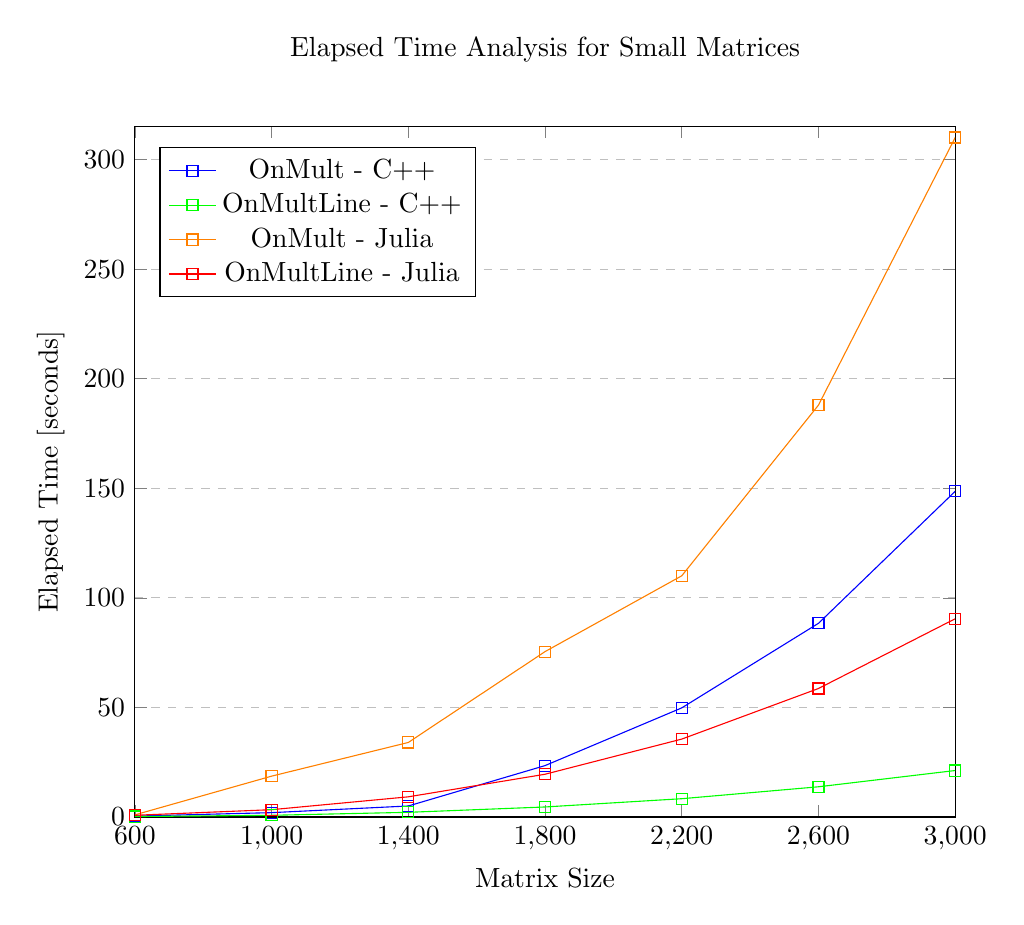
\begin{tikzpicture}
    \begin{axis}[
        title={Elapsed Time Analysis for Small Matrices},
        xlabel={Matrix Size},
        ylabel={Elapsed Time [seconds]},
        xmin=600, xmax=3000,
        ymin=0, ymax=315,
        xtick={600,1000,1400,1800,2200,2600,3000},
        legend pos=north west,
        ymajorgrids=true,
        grid style=dashed,
    ]
        \addplot[
            color=blue,
            mark=square,
            ]
            coordinates {
                (600,0.43)
                (1000,2.01)
                (1400,5.05)
                (1800,23.47)
                (2200,49.81)
                (2600,88.4)
                (3000,148.62)
            };
        \addlegendentry{OnMult - C++}
        \addplot[
            color=green,
            mark=square,
            ]
            coordinates {
                (600,0.23)
                (1000,0.8)
                (1400,2.16)
                (1800,4.6)
                (2200,8.37)
                (2600,13.81)
                (3000,21.23)
            };
        \addlegendentry{OnMultLine - C++}
        \addplot[
            color=orange,
            mark=square,
            ]
            coordinates {
                (600,1)
                (1000,18.66)
                (1400,34.03)
                (1800,75.48)
                (2200,110.07)
                (2600,187.95)
                (3000,310.04)
            };
        \addlegendentry{OnMult - Julia}
        \addplot[
            color=red,
            mark=square,
            ]
            coordinates {
                (600,0.81)
                (1000,3.36)
                (1400,9.23)
                (1800,19.53)
                (2200,35.57)
                (2600,58.65)
                (3000,90.47)
            };
        \addlegendentry{OnMultLine - Julia}
    \end{axis}
\end{tikzpicture}
\noindent\rule{\textwidth}{1pt}

% ==================================================================== 
% Level 1 Data Cache Misses Analysis for Small Matrices
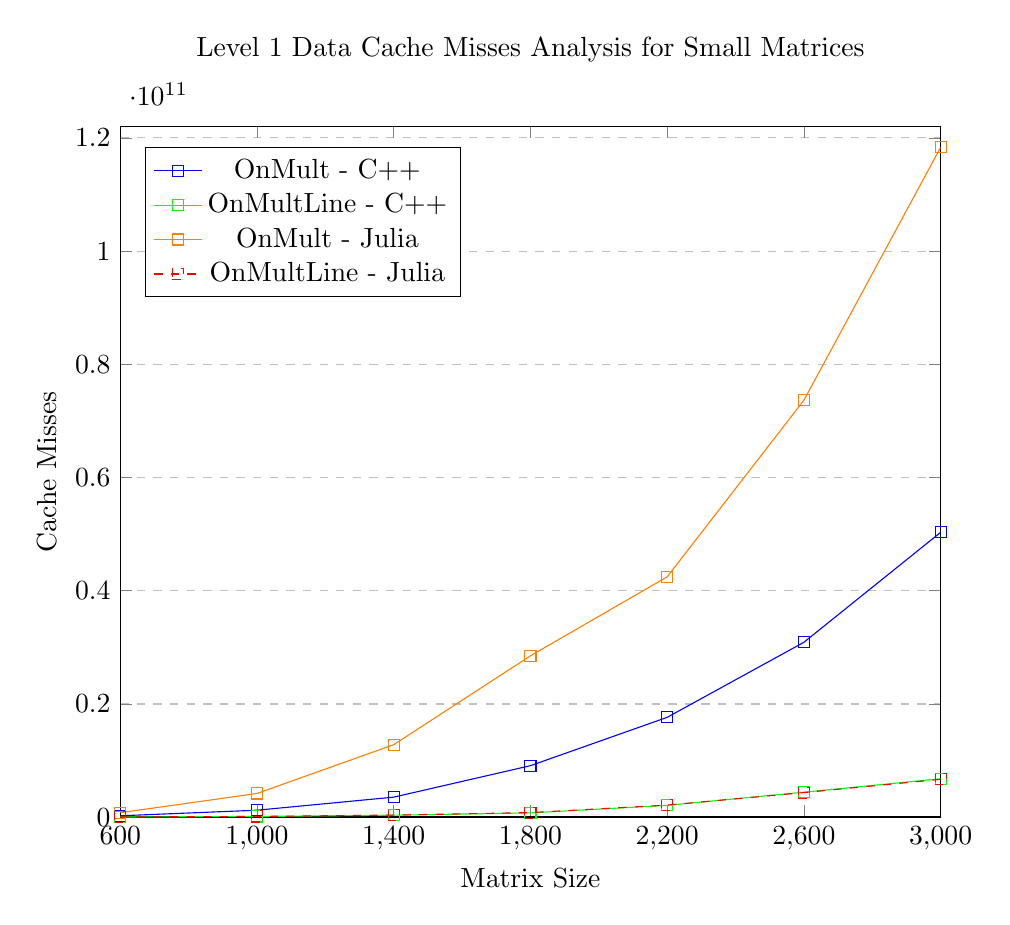
\begin{tikzpicture}
    \begin{axis}[
        title={Level 1 Data Cache Misses Analysis for Small Matrices},
        xlabel={Matrix Size},
        ylabel={Cache Misses},
        xmin=600, xmax=3000,
        ymin=20000000, ymax=122000000000,
        xtick={600,1000,1400,1800,2200,2600,3000},
        legend pos=north west,
        ymajorgrids=true,
        grid style=dashed,
    ]
        \addplot[
            color=blue,
            mark=square,
            ]
            coordinates {
                (600,242642372)
                (1000,1228764556)
                (1400,3537193200)
                (1800,9096697561)
                (2200,17636955944)
                (2600,30894833152)
                (3000,50317470107)
            };
        \addlegendentry{OnMult - C++}
        \addplot[
            color=green,
            mark=square,
            ]
            coordinates {
                (600,27391680)
                (1000,126233578)
                (1400,347827988)
                (1800,754741945)
                (2200,2087751131)
                (2600,4413206149)
                (3000,6780866661)
            };
        \addlegendentry{OnMultLine - C++}
        \addplot[
            color=orange,
            mark=square,
            ]
            coordinates {
                (600,790500038)
                (1000,4187023004)
                (1400,12802856300)
                (1800,28503048692)
                (2200,42455586813)
                (2600,73649099522)
                (3000,118329112126)
            };
        \addlegendentry{OnMult - Julia}
        \addplot[
            dashed,
            color=red,
            mark=square,
            ]
            coordinates {
                (600,28243918)
                (1000,127559089)
                (1400,365215495)
                (1800,806489775)
                (2200,2130800409)
                (2600,4342081165)
                (3000,6687741740)
            };
        \addlegendentry{OnMultLine - Julia}
    \end{axis}
\end{tikzpicture}
\noindent\rule{\textwidth}{1pt}

% ====================================================================
% Level 2 Data Cache Misses Analysis for Small Matrices
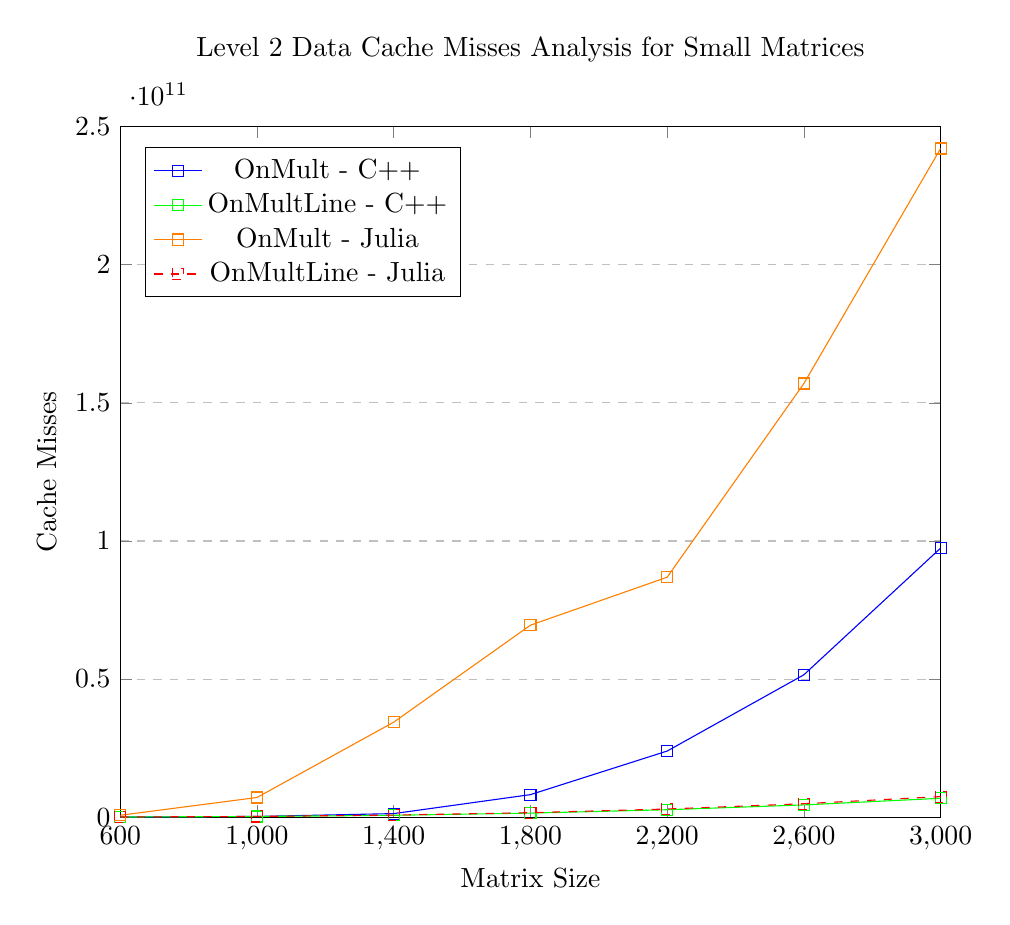
\begin{tikzpicture}
    \begin{axis}[
        title={Level 2 Data Cache Misses Analysis for Small Matrices},
        xlabel={Matrix Size},
        ylabel={Cache Misses},
        xmin=600, xmax=3000,
        ymin=50000000, ymax=250000000000,
        xtick={600,1000,1400,1800,2200,2600,3000},
        legend pos=north west,
        ymajorgrids=true,
        grid style=dashed,
    ]
        \addplot[
            color=blue,
            mark=square,
            ]
            coordinates {
                (600,38201753)
                (1000,265740919)
                (1400,1295805616)
                (1800,8165088643)
                (2200,23942351987)
                (2600,51560197814)
                (3000,97414965879)
            };
        \addlegendentry{OnMult - C++}
        \addplot[
            color=green,
            mark=square,
            ]
            coordinates {
                (600,55616260)
                (1000,252228230)
                (1400,690975001)
                (1800,1478164216)
                (2200,2700983098)
                (2600,4450312355)
                (3000,6844537009)
            };
        \addlegendentry{OnMultLine - C++}
        \addplot[
            color=orange,
            mark=square,
            ]
            coordinates {
                (600,691933900)
                (1000,7128452731)
                (1400,34399044658)
                (1800,69504279682)
                (2200,86876310308)
                (2600,157002737331)
                (3000,242074374008)
            };
        \addlegendentry{OnMult - Julia}
        \addplot[
            dashed,
            color=red,
            mark=square,
            ]
            coordinates {
                (600,60079868)
                (1000,276311056)
                (1400,768173019)
                (1800,1634536964)
                (2200,2961348844)
                (2600,4881135576)
                (3000,7457459209)
            };
        \addlegendentry{OnMultLine - Julia}
    \end{axis}
\end{tikzpicture}
\noindent\rule{\textwidth}{1pt}

% ====================================================================
% Total Instructions Completed Analysis for Small Matrices
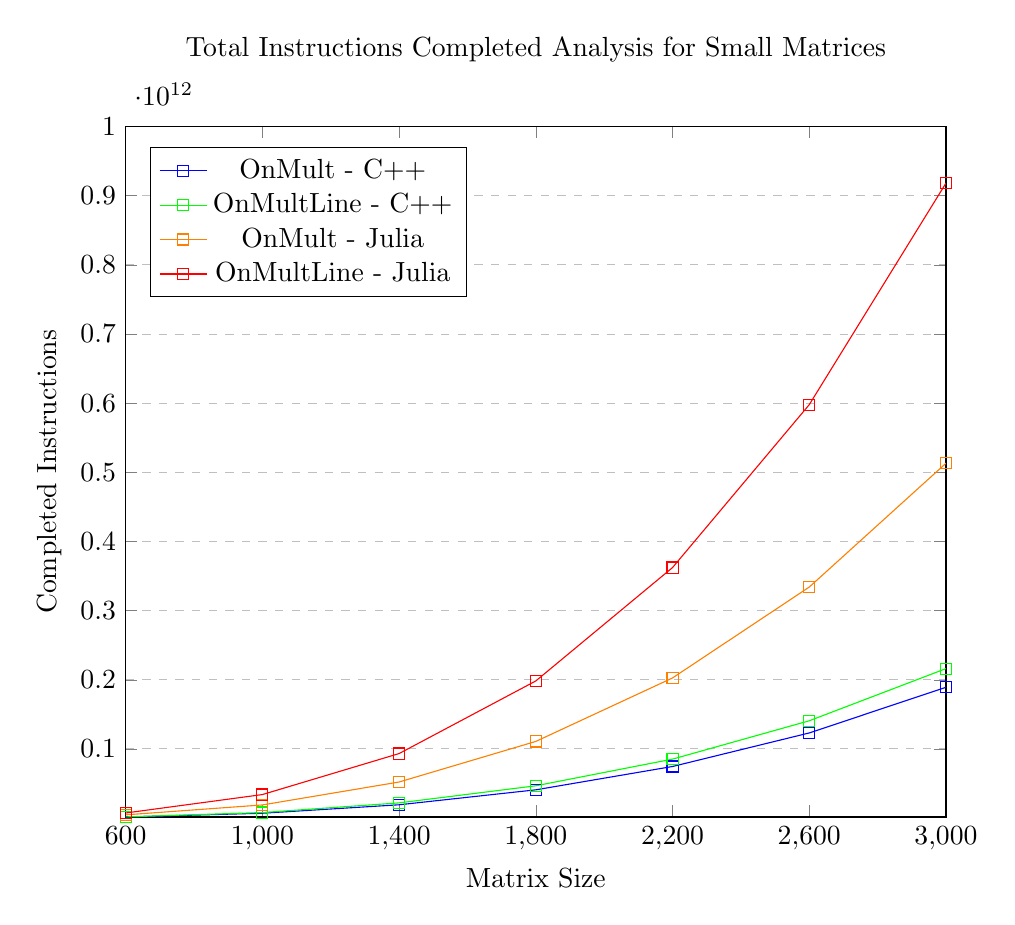
\begin{tikzpicture}
    \begin{axis}[
        title={Total Instructions Completed Analysis for Small Matrices},
        xlabel={Matrix Size},
        ylabel={Completed Instructions},
        xmin=600, xmax=3000,
        ymin=1500000000, ymax=1000000000000,
        xtick={600,1000,1400,1800,2200,2600,3000},
        legend pos=north west,
        ymajorgrids=true,
        grid style=dashed,
    ]
        \addplot[
            color=blue,
            mark=square,
            ]
            coordinates {
                (600,1518205115)
                (1000,7017111716)
                (1400,19241461015)
                (1800,40879260140)
                (2200,74618500388)
                (2600,123147182907)
                (3000,189153318019)
            };
        \addlegendentry{OnMult - C++}
        \addplot[
            color=green,
            mark=square,
            ]
            coordinates {
                (600,1735286324)
                (1000,8020111511)
                (1400,21991339535)
                (1800,46720971486)
                (2200,85281004166)
                (2600,140743440779)
                (3000,216180278092)
            };
        \addlegendentry{OnMultLine - C++}
        \addplot[
            color=orange,
            mark=square,
            ]
            coordinates {
                (600,4684283242)
                (1000,19020140154)
                (1400,52177868671)
                (1800,110872142893)
                (2200,202675645199)
                (2600,334098031635)
                (3000,513196185174)
            };
        \addlegendentry{OnMult - Julia}
        \addplot[
            color=red,
            mark=square,
            ]
            coordinates {
                (600,7369559576)
                (1000,34021060921)
                (1400,93315824848)
                (1800,198341345353)
                (2200,362325497017)
                (2600,597894187134)
                (3000,918329786996)
            };
        \addlegendentry{OnMultLine - Julia}
    \end{axis}
\end{tikzpicture}
\noindent\rule{\textwidth}{1pt}

% ====================================================================
% Total Cycles Analysis for Small Matrices
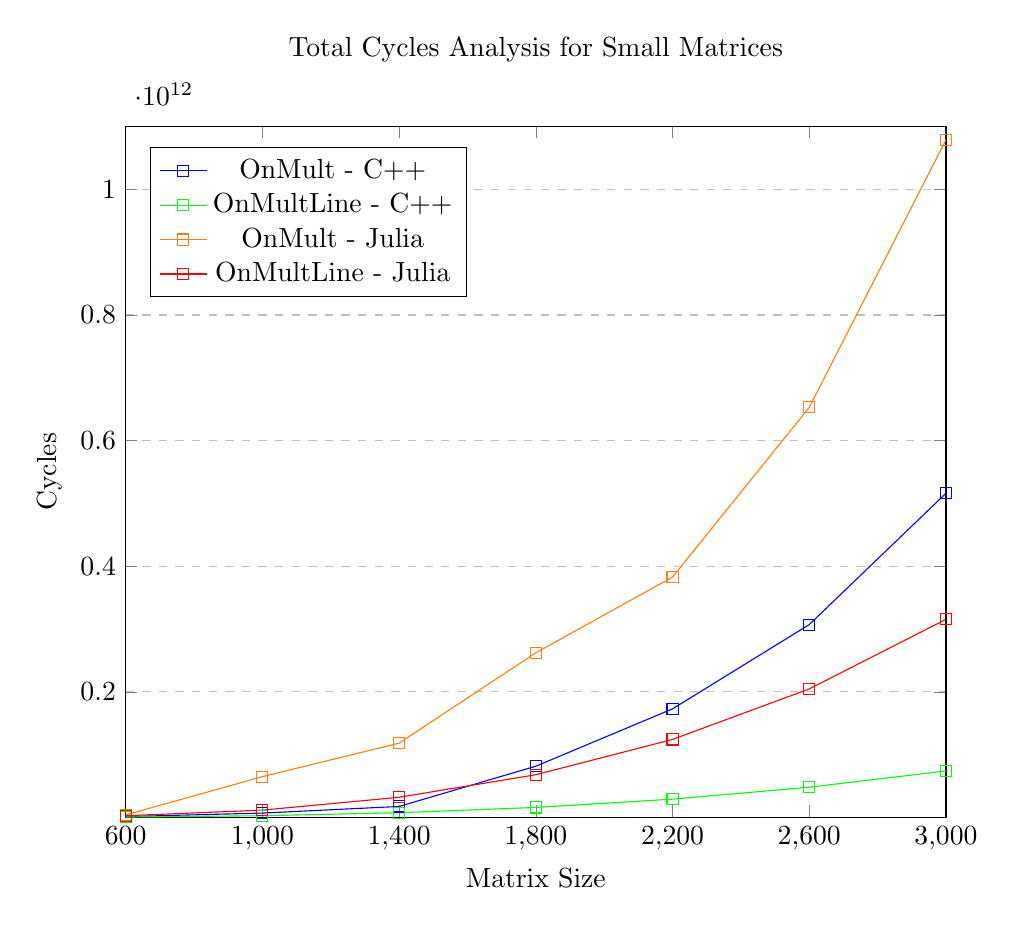
\begin{tikzpicture}
    \begin{axis}[
        title={Total Cycles Analysis for Small Matrices},
        xlabel={Matrix Size},
        ylabel={Cycles},
        xmin=600, xmax=3000,
        ymin=700000000, ymax=1100000000000,
        xtick={600,1000,1400,1800,2200,2600,3000},
        legend pos=north west,
        ymajorgrids=true,
        grid style=dashed,
    ]
        \addplot[
            color=blue,
            mark=square,
            ]
            coordinates {
                (600,1453882239)
                (1000,7020660831)
                (1400,17589029909)
                (1800,81656711071)
                (2200,172955210804)
                (2600,307124380544)
                (3000,516259930075)
            };
        \addlegendentry{OnMult - C++}
        \addplot[
            color=green,
            mark=square,
            ]
            coordinates {
                (600,731568849)
                (1000,2796360303)
                (1400,7548688815)
                (1800,16054568787)
                (2200,29225515050)
                (2600,48215845000)
                (3000,74100730666)
            }; 
        \addlegendentry{OnMultLine - C++}
        \addplot[
            color=orange,
            mark=square,
            ]
            coordinates {
                (600,4071759179)
                (1000,65019318867)
                (1400,118322522816)
                (1800,262195836378)
                (2200,382813539405)
                (2600,652962498386)
                (3000,1079053093367)
            };
        \addlegendentry{OnMult - Julia}
        \addplot[
            color=red,
            mark=square,
            ]
            coordinates {
                (600,2774567683)
                (1000,11728010137)
                (1400,32180992811)
                (1800,68087610615)
                (2200,124264821502)
                (2600,204721349139)
                (3000,315527429224)
            };
        \addlegendentry{OnMultLine - Julia}
    \end{axis}
\end{tikzpicture}
\noindent\rule{\textwidth}{1pt}

% ====================================================================
%                           Big Matrices
% ====================================================================

% ====================================================================
% Elapsed Time Analysis for Big Matrices
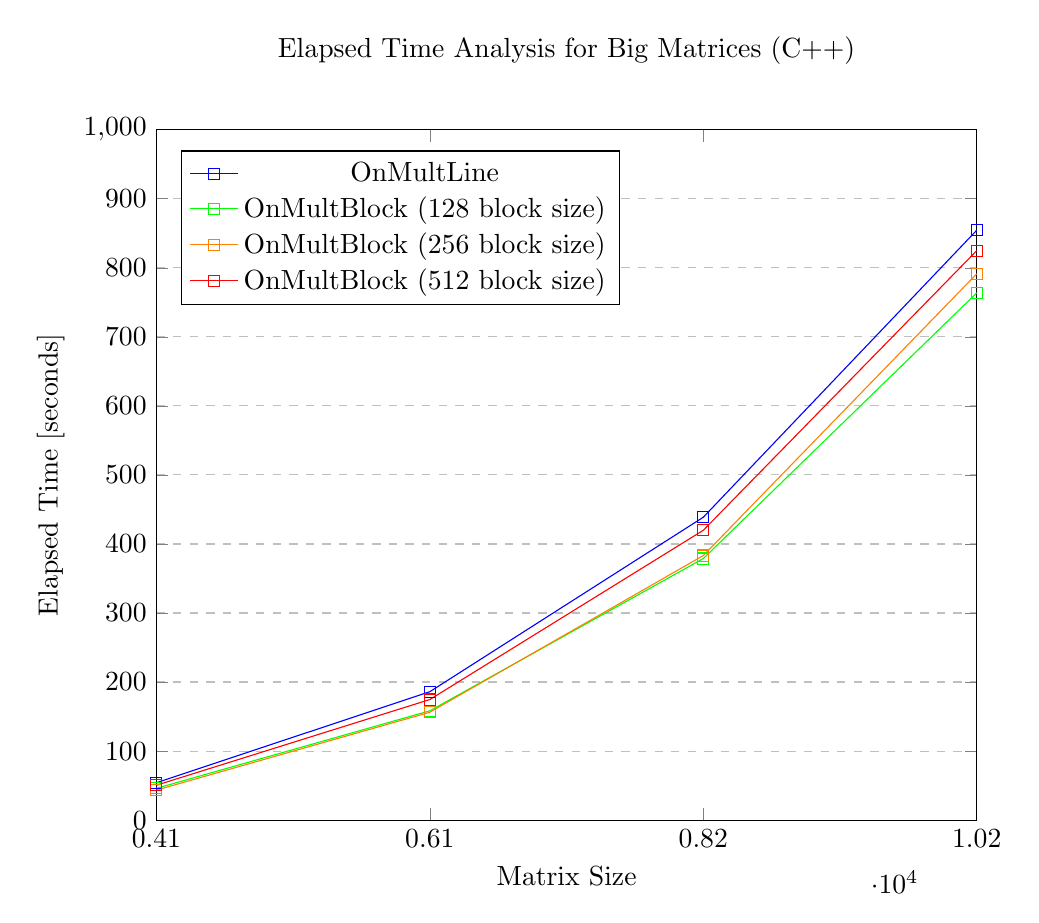
\begin{tikzpicture}
    \begin{axis}[
        title={Elapsed Time Analysis for Big Matrices (C++)},
        xlabel={Matrix Size},
        ylabel={Elapsed Time [seconds]},
        xmin=4096, xmax=10240,
        ymin=0, ymax=1000,
        xtick={4096,6144,8192,10240},
        legend pos=north west,
        ymajorgrids=true,
        grid style=dashed,
    ]
        \addplot[
            color=blue,
            mark=square,
            ]
            coordinates {
                (4096,54.2)
                (6144,186.02)
                (8192,438.7)
                (10240,854.4)
            };
        \addlegendentry{OnMultLine}
        \addplot[
            color=green,
            mark=square,
            ]
            coordinates {
                (4096,46.06)
                (6144,158.33)
                (8192,378.85)
                (10240,763.66)
            };
        \addlegendentry{OnMultBlock (128 block size)}
        \addplot[
            color=orange,
            mark=square,
            ]
            coordinates {
                (4096,43.48)
                (6144,156.26)
                (8192,383.22)
                (10240,791.27)
            };
        \addlegendentry{OnMultBlock (256 block size)}
        \addplot[
            color=red,
            mark=square,
            ]
            coordinates {
                (4096,50.57)
                (6144,174.66)
                (8192,419.81)
                (10240,824.83)
            };
        \addlegendentry{OnMultBlock (512 block size)}
    \end{axis}
\end{tikzpicture}
\noindent\rule{\textwidth}{1pt}

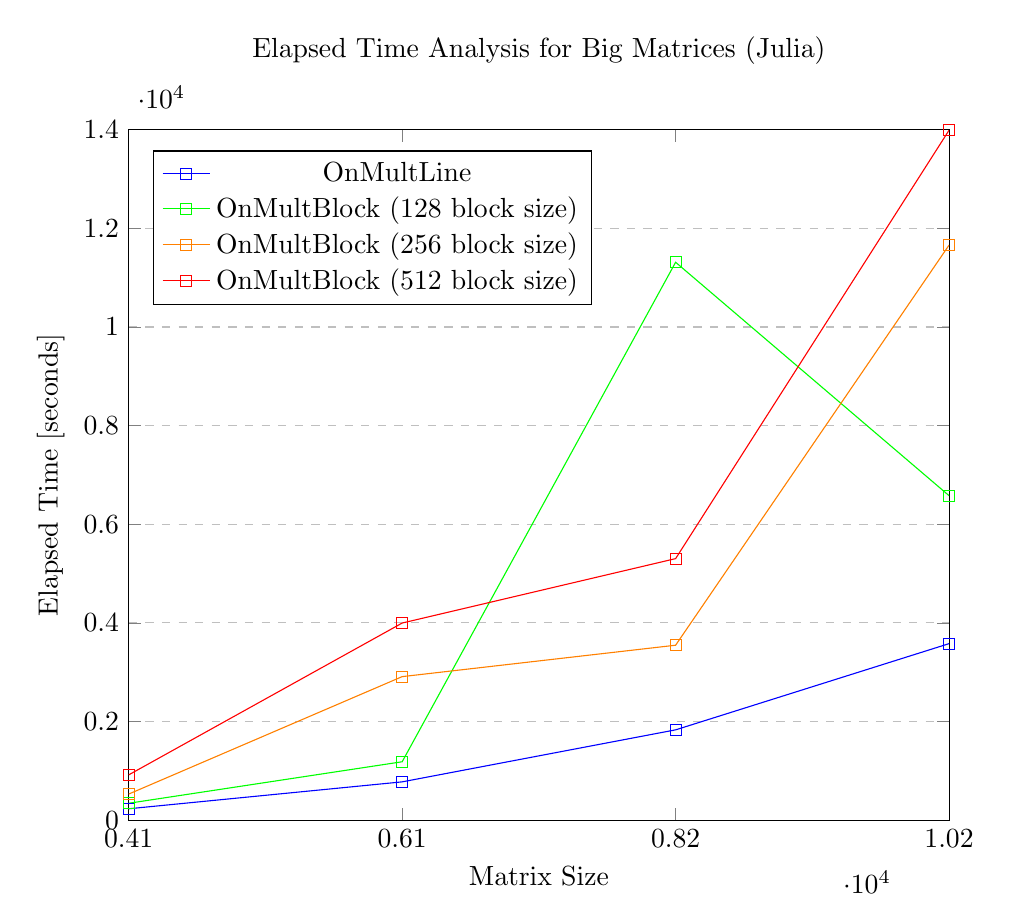
\begin{tikzpicture}
    \begin{axis}[
        title={Elapsed Time Analysis for Big Matrices (Julia)},
        xlabel={Matrix Size},
        ylabel={Elapsed Time [seconds]},
        xmin=4096, xmax=10240,
        ymin=0, ymax=14000,
        xtick={4096,6144,8192,10240},
        legend pos=north west,
        ymajorgrids=true,
        grid style=dashed,
    ]
        \addplot[
            color=blue,
            mark=square,
            ]
            coordinates {
                (4096,230.27)
                (6144,776.02)
                (8192,1830.69)
                (10240,3578.77)
            };
        \addlegendentry{OnMultLine}
        \addplot[
            color=green,
            mark=square,
            ]
            coordinates {
                (4096,341.96)
                (6144,1183.62)
                (8192,11312.07)
                (10240,6578.75)
            };
        \addlegendentry{OnMultBlock (128 block size)}
        \addplot[
            color=orange,
            mark=square,
            ]
            coordinates {
                (4096,528.44)
                (6144,2909.77)
                (8192,3546.83)
                (10240,11660.25)
            };
        \addlegendentry{OnMultBlock (256 block size)}
        \addplot[
            color=red,
            mark=square,
            ]
            coordinates {
                (4096,917.71)
                (6144,3996.44)
                (8192,5302.64)
                (10240,13989.91)
            };
        \addlegendentry{OnMultBlock (512 block size)}
    \end{axis}
\end{tikzpicture}
\noindent\rule{\textwidth}{1pt}

% ====================================================================
% Level 1 Data Cache Misses Analysis for Big Matrices
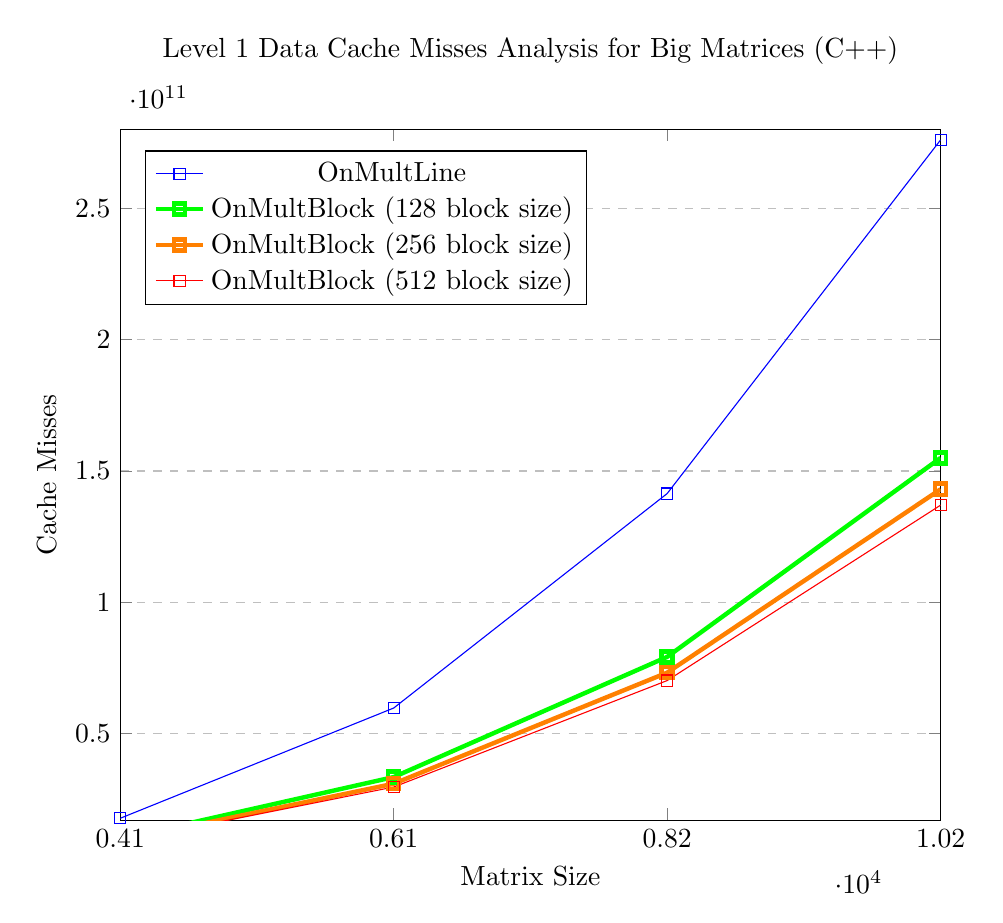
\begin{tikzpicture}
    \begin{axis}[
        title={Level 1 Data Cache Misses Analysis for Big Matrices (C++)},
        xlabel={Matrix Size},
        ylabel={Cache Misses},
        xmin=4096, xmax=10240,
        ymin=17000000000, ymax=280000000000,
        xtick={4096,6144,8192,10240},
        legend pos=north west,
        ymajorgrids=true,
        grid style=dashed,
    ]
        \addplot[
            color=blue,
            mark=square,
            ]
            coordinates {
                (4096,17707708096)
                (6144,59702012040)
                (8192,141401440293)
                (10240,276115987181)
            };
        \addlegendentry{OnMultLine}
        \addplot[
            style={ultra thick},
            color=green,
            mark=square,
            ]
            coordinates {
                (4096,9916460516)
                (6144,33405907798)
                (8192,79181095635)
                (10240,154996090380)
            };
        \addlegendentry{OnMultBlock (128 block size)}
        \addplot[
            style={ultra thick},
            color=orange,
            mark=square,
            ]
            coordinates {
                (4096,9149861272)
                (6144,30869068549)
                (8192,73171911624)
                (10240,143046520843)
            };
        \addlegendentry{OnMultBlock (256 block size)}
        \addplot[
            color=red,
            mark=square,
            ]
            coordinates {
                (4096,8760458941)
                (6144,29605757450)
                (8192,70164130068)
                (10240,136988329116)
            };
        \addlegendentry{OnMultBlock (512 block size)}
    \end{axis}
\end{tikzpicture}
\noindent\rule{\textwidth}{1pt}

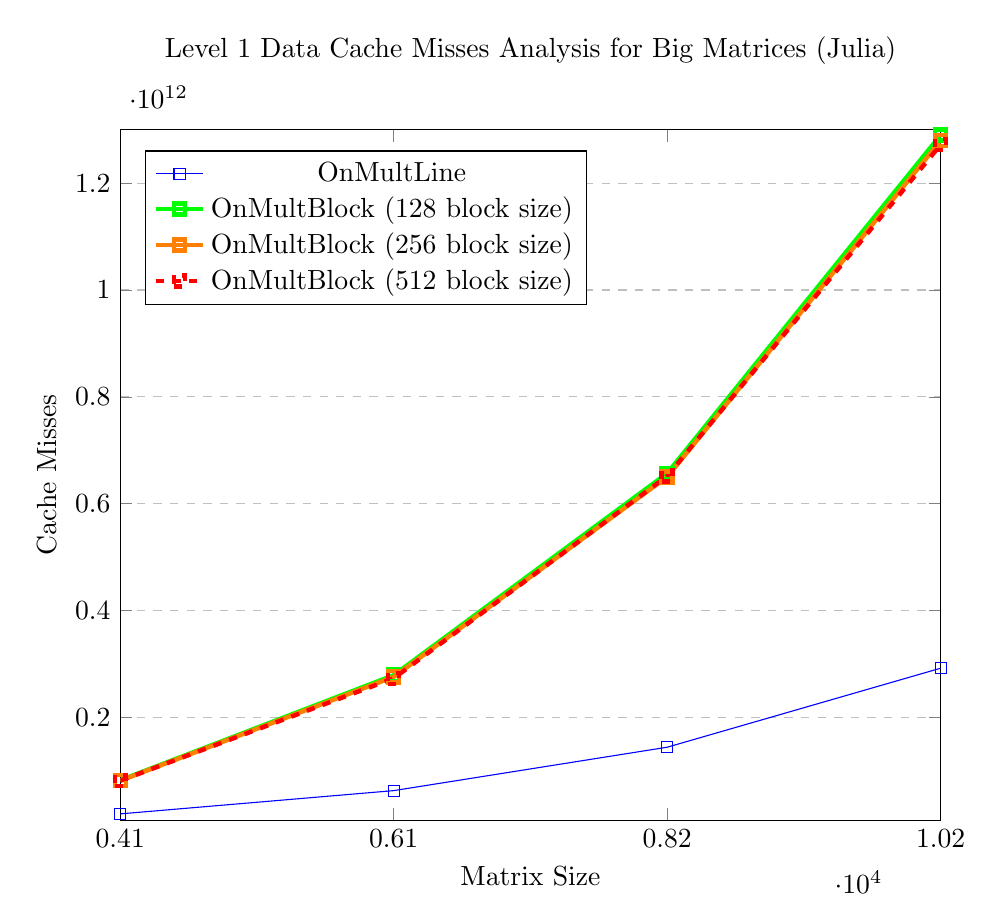
\begin{tikzpicture}
    \begin{axis}[
        title={Level 1 Data Cache Misses Analysis for Big Matrices (Julia)},
        xlabel={Matrix Size},
        ylabel={Cache Misses},
        xmin=4096, xmax=10240,
        ymin=8000000000, ymax=1300000000000,
        xtick={4096,6144,8192,10240},
        legend pos=north west,
        ymajorgrids=true,
        grid style=dashed,
    ]
        \addplot[
            color=blue,
            mark=square,
            ]
            coordinates {
                (4096,19683275358)
                (6144,63209788326)
                (8192,144436936126)
                (10240,292269153834)
            };
        \addlegendentry{OnMultLine}
        \addplot[
            style={ultra thick},
            color=green,
            mark=square,
            ]
            coordinates {
                (4096,82575870462)
                (6144,279174675676)
                (8192,656983569809)
                (10240,1290008318948)
            };
        \addlegendentry{OnMultBlock (128 block size)}
        \addplot[
            style={ultra thick},
            color=orange,
            mark=square,
            ]
            coordinates {
                (4096,81807718147)
                (6144,276170798019)
                (8192,650322395623)
                (10240,1279557730274)
            };
        \addlegendentry{OnMultBlock (256 block size)}
        \addplot[
            style={ultra thick},
            dashed,
            color=red,
            mark=square,
            ]
            coordinates {
                (4096,81759064227)
                (6144,273384517535)
                (8192,651756808874)
                (10240,1271856376836)
            };
        \addlegendentry{OnMultBlock (512 block size)}
    \end{axis}
\end{tikzpicture}
\noindent\rule{\textwidth}{1pt}

% ====================================================================
% Level 2 Data Cache Misses Analysis for Big Matrices
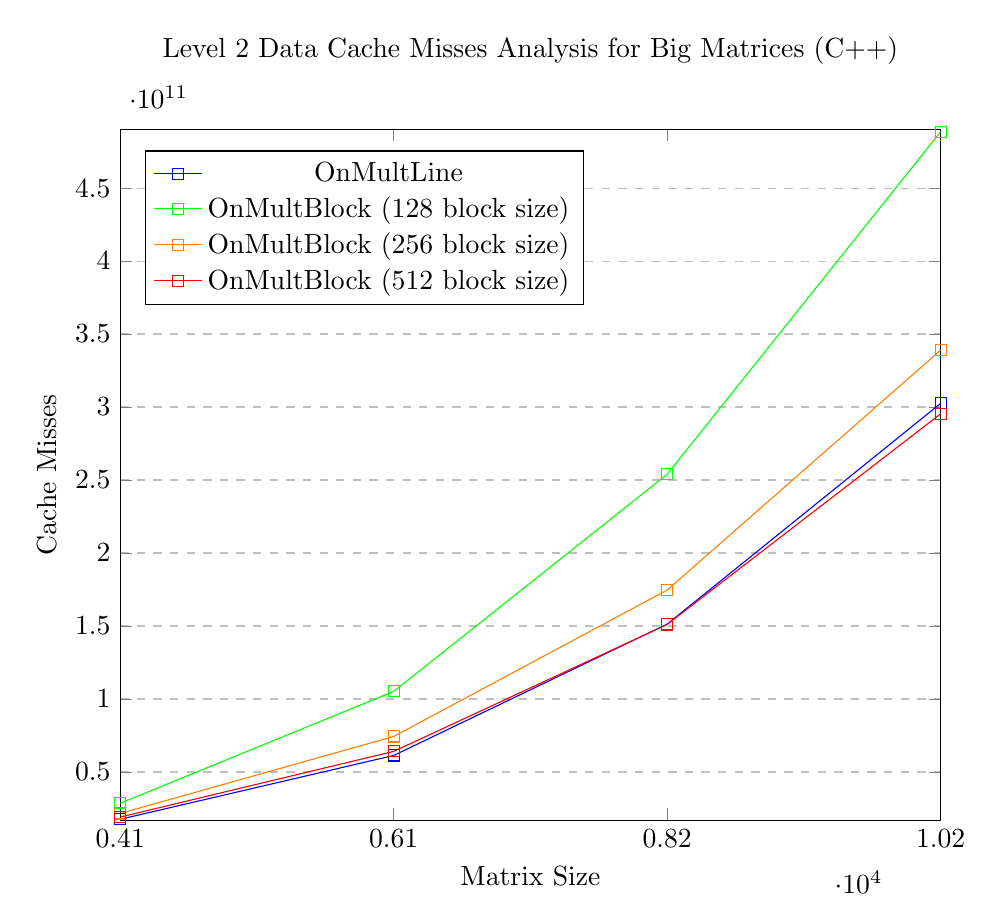
\begin{tikzpicture}
    \begin{axis}[
        title={Level 2 Data Cache Misses Analysis for Big Matrices (C++)},
        xlabel={Matrix Size},
        ylabel={Cache Misses},
        xmin=4096, xmax=10240,
        ymin=17000000000, ymax=490000000000,
        xtick={4096,6144,8192,10240},
        legend pos=north west,
        ymajorgrids=true,
        grid style=dashed,
    ]
        \addplot[
            color=blue,
            mark=square,
            ]
            coordinates {
                (4096,17586042367)
                (6144,61303190917)
                (8192,151295111884)
                (10240,302496619366)
            };
        \addlegendentry{OnMultLine}
        \addplot[
            color=green,
            mark=square,
            ]
            coordinates {
                (4096,28566608428)
                (6144,105196803686)
                (8192,253956049179)
                (10240,488560986796)
            };
        \addlegendentry{OnMultBlock (128 block size)}
        \addplot[
            color=orange,
            mark=square,
            ]
            coordinates {
                (4096,21603105776)
                (6144,74314991708)
                (8192,174616538353)
                (10240,338989773582)
            };
        \addlegendentry{OnMultBlock (256 block size)}
        \addplot[
            color=red,
            mark=square,
            ]
            coordinates {
                (4096,19114338033)
                (6144,64111369915)
                (8192,151077531631)
                (10240,295313892131)
            };         
        \addlegendentry{OnMultBlock (512 block size)}
    \end{axis}
\end{tikzpicture}
\noindent\rule{\textwidth}{1pt}

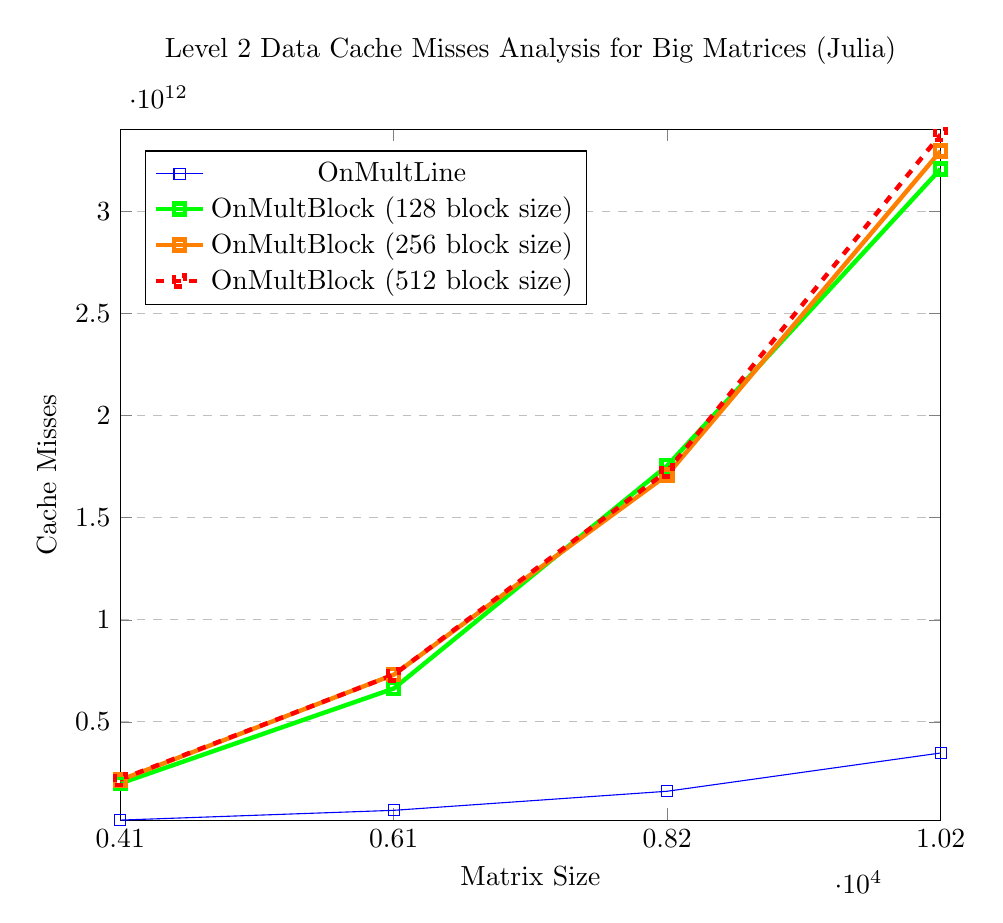
\begin{tikzpicture}
    \begin{axis}[
        title={Level 2 Data Cache Misses Analysis for Big Matrices (Julia)},
        xlabel={Matrix Size},
        ylabel={Cache Misses},
        xmin=4096, xmax=10240,
        ymin=19000000000, ymax=3400000000000,
        xtick={4096,6144,8192,10240},
        legend pos=north west,
        ymajorgrids=true,
        grid style=dashed,
    ]
        \addplot[
            color=blue,
            mark=square,
            ]
            coordinates {
                (4096,19089020846)
                (6144,67008304574)
                (8192,160418112547)
                (10240,347788413251)
            };
        \addlegendentry{OnMultLine}
        \addplot[
            style={ultra thick},
            color=green,
            mark=square,
            ]
            coordinates {
                (4096,198605733564)
                (6144,663340116145)
                (8192,1754318635889)
                (10240,3208053644364)
            };         
        \addlegendentry{OnMultBlock (128 block size)}
        \addplot[
            style={ultra thick},
            color=orange,
            mark=square,
            ]
            coordinates {
                (4096,215206777299)
                (6144,731187468609)
                (8192,1709268086391)
                (10240,3295688081895)
            };
        \addlegendentry{OnMultBlock (256 block size)}
        \addplot[
            style={ultra thick},
            dashed,
            color=red,
            mark=square,
            ]
            coordinates {
                (4096,218180831230)
                (6144,730836112361)
                (8192,1727985459300)
                (10240,3376247779332)
            };
        \addlegendentry{OnMultBlock (512 block size)}
    \end{axis}
\end{tikzpicture}
\noindent\rule{\textwidth}{1pt}

% ====================================================================
% Total Instructions Completed Analysis for Big Matrices
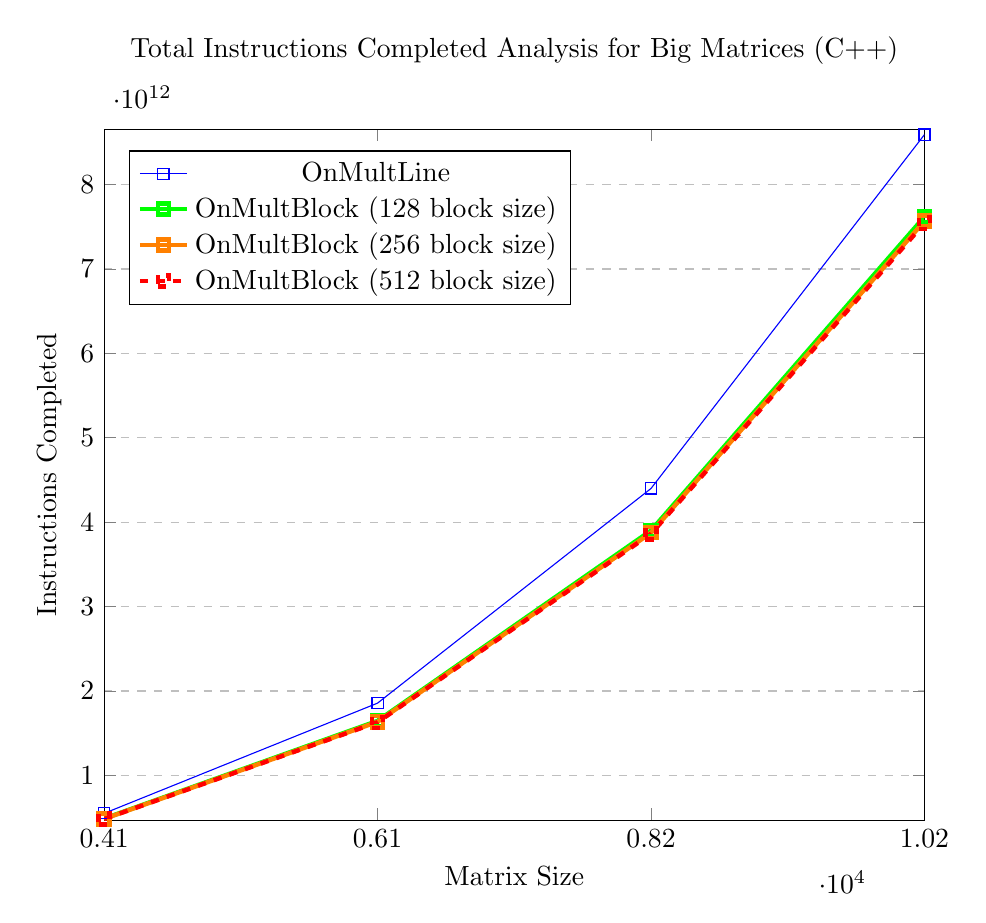
\begin{tikzpicture}
    \begin{axis}[
        title={Total Instructions Completed Analysis for Big Matrices (C++)},
        xlabel={Matrix Size},
        ylabel={Instructions Completed},
        xmin=4096, xmax=10240,
        ymin=470000000000, ymax=8650000000000,
        xtick={4096,6144,8192,10240},
        legend pos=north west,
        ymajorgrids=true,
        grid style=dashed,
    ]
        \addplot[
            color=blue,
            mark=square,
            ]
            coordinates {
                (4096,550091753257)
                (6144,1856181522841)
                (8192,4399389720695)
                (10240,8592033218858)
            };         
        \addlegendentry{OnMultLine}
        \addplot[
            style={ultra thick},
            color=green,
            mark=square,
            ]
            coordinates {
                (4096,487672443536)
                (6144,1645742915859)
                (8192,3900840784634)
                (10240,7618619462282)
            };
        \addlegendentry{OnMultBlock (128 block size)}
        \addplot[
            style={ultra thick},
            color=orange,
            mark=square,
            ]
            coordinates {
                (4096,484406853030)
                (6144,1634721559533)
                (8192,3874716111168)
                (10240,7567594712008)
            };
        \addlegendentry{OnMultBlock (256 block size)}
        \addplot[
            dashed,
            style={ultra thick},
            color=red,
            mark=square,
            ]
            coordinates {
                (4096,482785191506)
                (6144,1629248449858)
                (8192,3861742800472)
                (10240,7542256231146)
            };         
        \addlegendentry{OnMultBlock (512 block size)}
    \end{axis}
\end{tikzpicture}
\noindent\rule{\textwidth}{1pt}

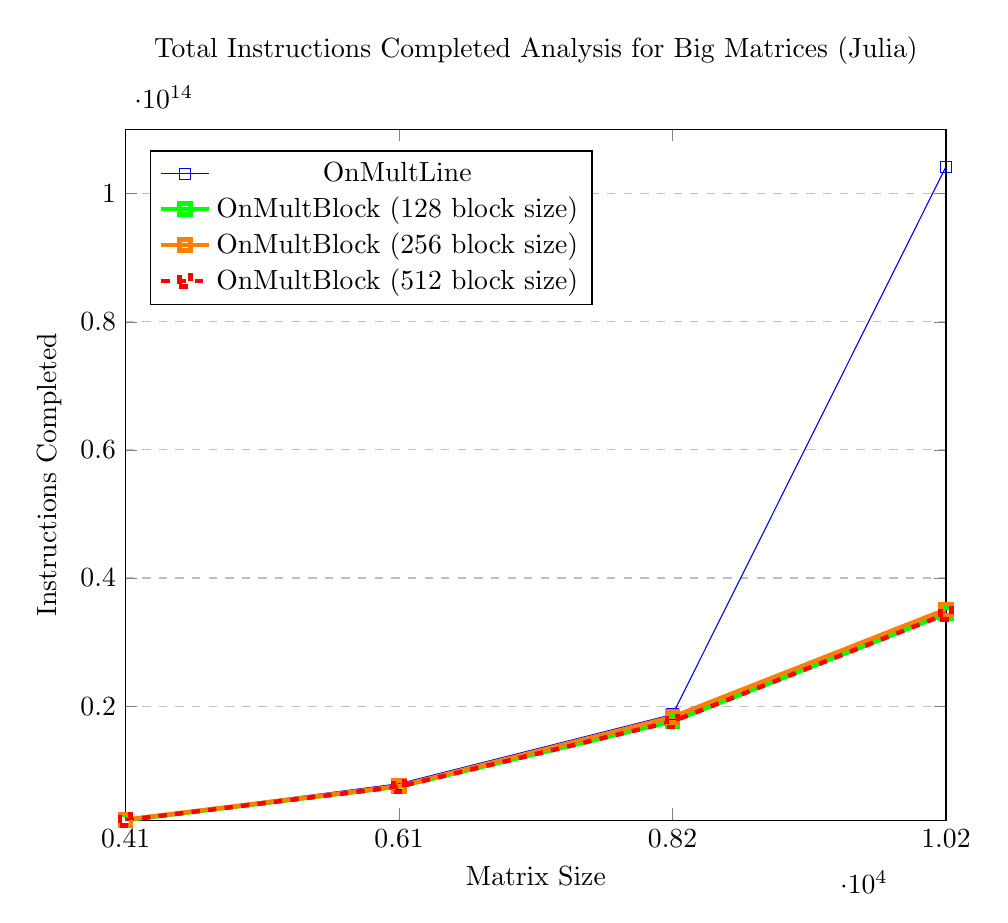
\begin{tikzpicture}
    \begin{axis}[
        title={Total Instructions Completed Analysis for Big Matrices (Julia)},
        xlabel={Matrix Size},
        ylabel={Instructions Completed},
        xmin=4096, xmax=10240,
        ymin=2200000000000, ymax=110000000000000,
        xtick={4096,6144,8192,10240},
        legend pos=north west,
        ymajorgrids=true,
        grid style=dashed,
    ]
        \addplot[
            color=blue,
            mark=square,
            ]
            coordinates {
                (4096,2336637413950)
                (6144,7886164756473)
                (8192,18692311790874)
                (10240,104229324721945)
            };
        \addlegendentry{OnMultLine}
        \addplot[
            style={ultra thick},
            color=green,
            mark=square,
            ]
            coordinates {
                (4096,2203642093822)
                (6144,7436680533958)
                (8192,17627885759912)
                (10240,34428131201672)
            };         
        \addlegendentry{OnMultBlock (128 block size)}
        \addplot[
            style={ultra thick},
            color=orange,
            mark=square,
            ]
            coordinates {
                (4096,2271203253286)
                (6144,7499059221580)
                (8192,18309808691882)
                (10240,35094145084977)
            };
        \addlegendentry{OnMultBlock (256 block size)}
        \addplot[
            style={ultra thick},
            dashed,
            color=red,
            mark=square,
            ]
            coordinates {
                (4096,2200678680772)
                (6144,7425620321651)
                (8192,17601106365647)
                (10240,34377715221058)
            };
        \addlegendentry{OnMultBlock (512 block size)}
    \end{axis}
\end{tikzpicture}
\noindent\rule{\textwidth}{1pt}

% ====================================================================
% Total Cycles Analysis for Big Matrices
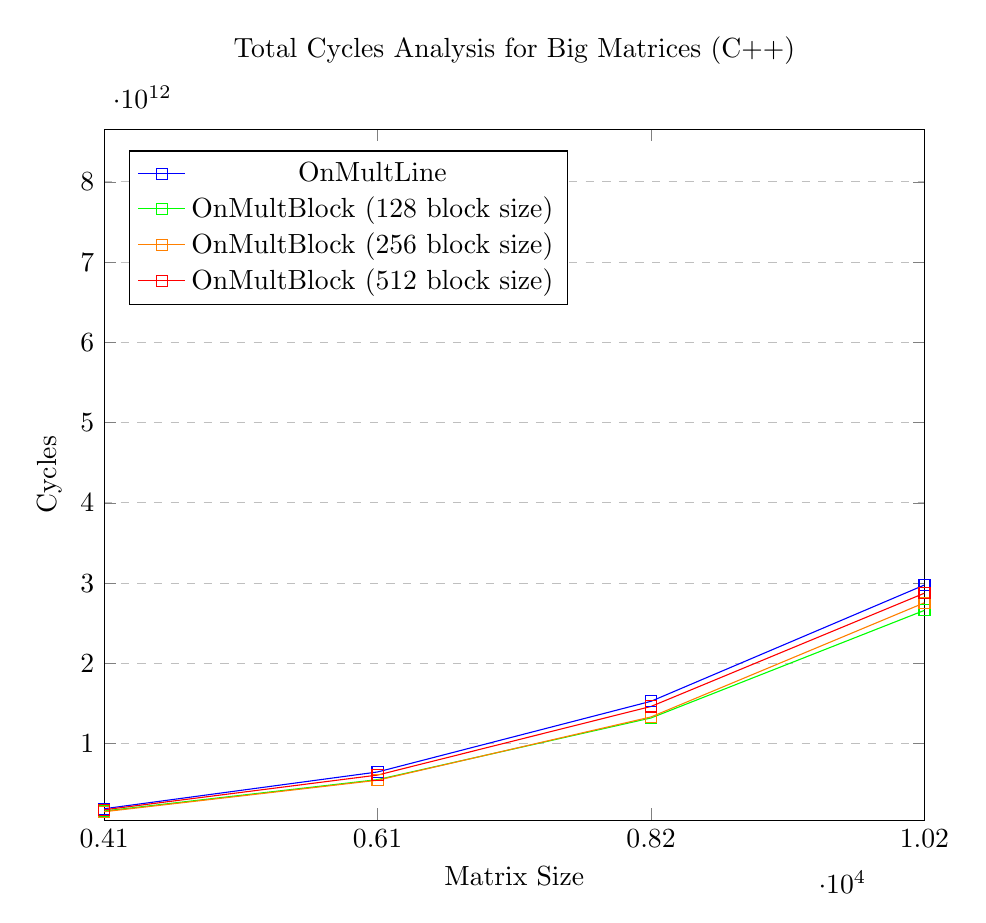
\begin{tikzpicture}
    \begin{axis}[
        title={Total Cycles Analysis for Big Matrices (C++)},
        xlabel={Matrix Size},
        ylabel={Cycles},
        xmin=4096, xmax=10240,
        ymin=47000000000, ymax=8650000000000,
        xtick={4096,6144,8192,10240},
        legend pos=north west,
        ymajorgrids=true,
        grid style=dashed,
    ]
        \addplot[
            color=blue,
            mark=square,
            ]
            coordinates {
                (4096,189055892334)
                (6144,647231640676)
                (8192,1528027963458)
                (10240,2976995283393)
            };         
        \addlegendentry{OnMultLine}
        \addplot[
            color=green,
            mark=square,
            ]
            coordinates {
                (4096,160753318010)
                (6144,551983745479)
                (8192,1320219014610)
                (10240,2660963658807)
            };
        \addlegendentry{OnMultBlock (128 block size)}
        \addplot[
            color=orange,
            mark=square,
            ]
            coordinates {
                (4096,151710235946)
                (6144,544202350886)
                (8192,1332982591971)
                (10240,2755506900596)
            };
        \addlegendentry{OnMultBlock (256 block size)}
        \addplot[
            color=red,
            mark=square,
            ]
            coordinates {
                (4096,176059851151)
                (6144,608680688714)
                (8192,1463688211485)
                (10240,2875262293733)
            };         
        \addlegendentry{OnMultBlock (512 block size)}
    \end{axis}
\end{tikzpicture}
\noindent\rule{\textwidth}{1pt}

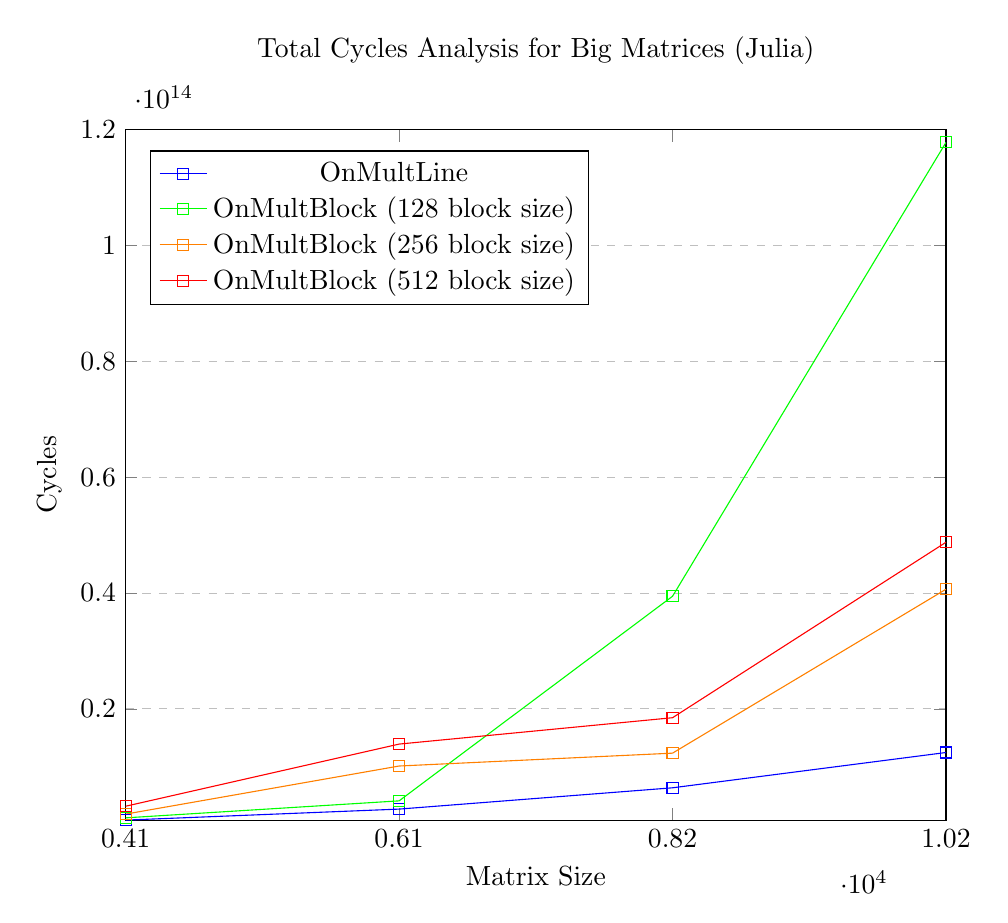
\begin{tikzpicture}
    \begin{axis}[
        title={Total Cycles Analysis for Big Matrices (Julia)},
        xlabel={Matrix Size},
        ylabel={Cycles},
        xmin=4096, xmax=10240,
        ymin=800000000000, ymax=120000000000000,
        xtick={4096,6144,8192,10240},
        legend pos=north west,
        ymajorgrids=true,
        grid style=dashed,
    ]
        \addplot[
            color=blue,
            mark=square,
            ]
            coordinates {
                (4096,802737212510)
                (6144,2704562199065)
                (8192,6381820595643)
                (10240,12474455554893)
            };
        \addlegendentry{OnMultLine}
        \addplot[
            color=green,
            mark=square,
            ]
            coordinates {
                (4096,1192439094684)
                (6144,4126471903572)
                (8192,39454835625174)
                (10240,117810311402863)
            };         
        \addlegendentry{OnMultBlock (128 block size)}
        \addplot[
            color=orange,
            mark=square,
            ]
            coordinates {
                (4096,1840867636066)
                (6144,10142125494224)
                (8192,12363647241767)
                (10240,40661598040956)
            };
        \addlegendentry{OnMultBlock (256 block size)}
        \addplot[
            color=red,
            mark=square,
            ]
            coordinates {
                (4096,3198640451343)
                (6144,13928558792091)
                (8192,18481224697344)
                (10240,48773210593815)
            };
        \addlegendentry{OnMultBlock (512 block size)}
    \end{axis}
\end{tikzpicture}
\noindent\rule{\textwidth}{1pt}

% ====================================================================
%                           Parallelization
% ====================================================================

% ====================================================================
% Elapsed Time Analysis for Parallelization

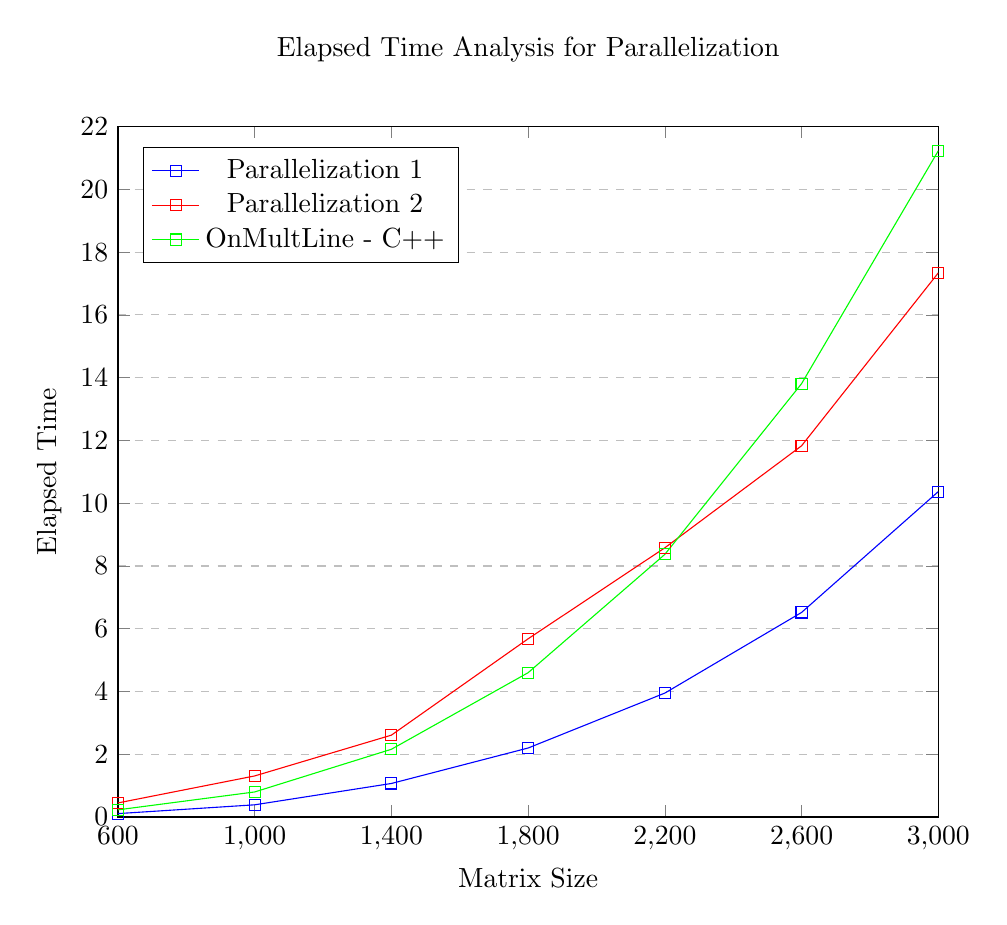
\begin{tikzpicture}
    \begin{axis}[
        title={Elapsed Time Analysis for Parallelization},
        xlabel={Matrix Size},
        ylabel={Elapsed Time},
        xmin=600, xmax=3000,
        ymin=0, ymax=22,
        xtick={600,1000,1400,1800,2200,2600,3000},
        legend pos=north west,
        ymajorgrids=true,
        grid style=dashed,
    ]
        \addplot[
            color=blue,
            mark=square,
            ]
            coordinates {
                (600,0.11)
                (1000,0.39)
                (1400,1.07)
                (1800,2.2)
                (2200,3.95)
                (2600,6.52)
                (3000,10.37)
            };
        \addlegendentry{Parallelization 1}
        \addplot[
            color=red,
            mark=square,
            ]
            coordinates {
                (600,0.45)
                (1000,1.31)
                (1400,2.61)
                (1800,5.68)
                (2200,8.58)
                (2600,11.83)
                (3000,17.34)
            };         
        \addlegendentry{Parallelization 2}
                \addplot[
            color=green,
            mark=square,
            ]
            coordinates {
                (600,0.23)
                (1000,0.8)
                (1400,2.16)
                (1800,4.6)
                (2200,8.37)
                (2600,13.81)
                (3000,21.23)
            };
        \addlegendentry{OnMultLine - C++}
    \end{axis}
\end{tikzpicture}
\noindent\rule{\textwidth}{1pt}

% ====================================================================
% Level 1 Data Cache Misses Analysis for Parallelization

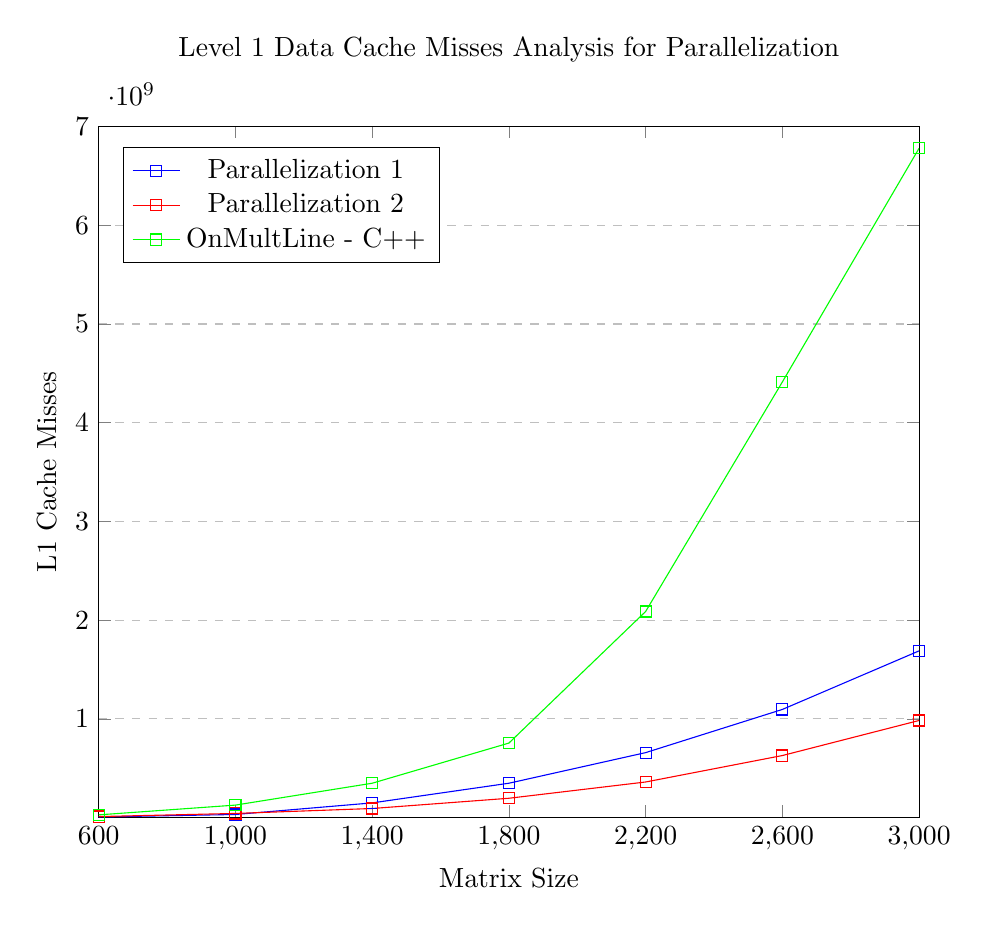
\begin{tikzpicture}
    \begin{axis}[
        title={Level 1 Data Cache Misses Analysis for Parallelization},
        xlabel={Matrix Size},
        ylabel={L1 Cache Misses},
        xmin=600, xmax=3000,
        ymin=5000000, ymax=7000000000,
        xtick={600,1000,1400,1800,2200,2600,3000},
        legend pos=north west,
        ymajorgrids=true,
        grid style=dashed,
    ]
        \addplot[
            color=blue,
            mark=square,
            ]
            coordinates {
                (600,5921060)
                (1000,31179542)
                (1400,148534995)
                (1800,347873725)
                (2200,657908228)
                (2600,1095357172)
                (3000,1688789073)
            };
        \addlegendentry{Parallelization 1}
        \addplot[
            color=red,
            mark=square,
            ]
            coordinates {
                (600,9976498)
                (1000,41697426)
                (1400,91833791)
                (1800,195569675)
                (2200,360346937)
                (2600,628339999)
                (3000,983510782)
            };         
        \addlegendentry{Parallelization 2}
                \addplot[
            color=green,
            mark=square,
            ]
            coordinates {
                (600,27391680)
                (1000,126233578)
                (1400,347827988)
                (1800,754741945)
                (2200,2087751131)
                (2600,4413206149)
                (3000,6780866661)
            };
        \addlegendentry{OnMultLine - C++}
    \end{axis}
\end{tikzpicture}
\noindent\rule{\textwidth}{1pt}

% ====================================================================
% Level 2 Data Cache Misses Analysis for Parallelization

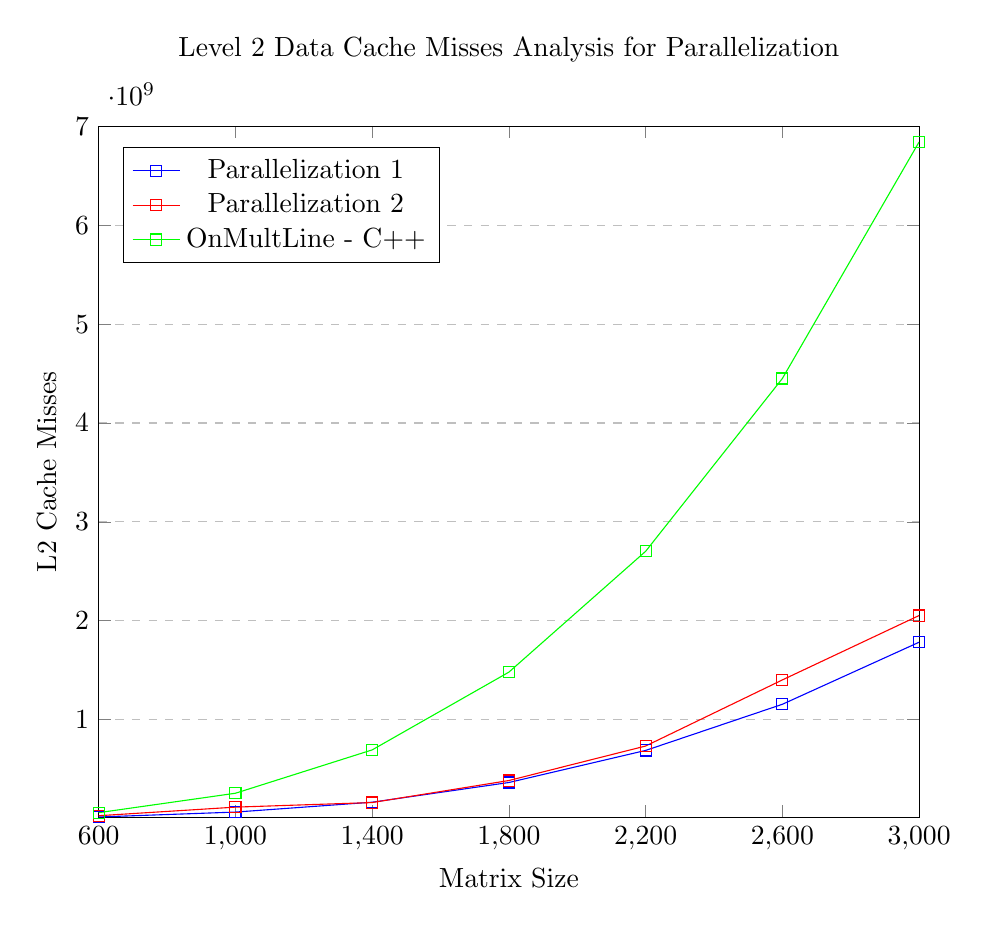
\begin{tikzpicture}
    \begin{axis}[
        title={Level 2 Data Cache Misses Analysis for Parallelization},
        xlabel={Matrix Size},
        ylabel={L2 Cache Misses},
        xmin=600, xmax=3000,
        ymin=11000000, ymax=7000000000,
        xtick={600,1000,1400,1800,2200,2600,3000},
        legend pos=north west,
        ymajorgrids=true,
        grid style=dashed,
    ]
        \addplot[
            color=blue,
            mark=square,
            ]
            coordinates {
                (600,11879142)
                (1000,61496962)
                (1400,161521723)
                (1800,360803027)
                (2200,685465656)
                (2600,1152601061)
                (3000,1780721781)
            };
        \addlegendentry{Parallelization 1}
        \addplot[
            color=red,
            mark=square,
            ]
            coordinates {
                (600,24803466)
                (1000,111586940)
                (1400,157959013)
                (1800,380947313)
                (2200,730171347)
                (2600,1399190595)
                (3000,2051038844)
            };         
        \addlegendentry{Parallelization 2}
                \addplot[
            color=green,
            mark=square,
            ]
            coordinates {
                (600,55616260)
                (1000,252228230)
                (1400,690975001)
                (1800,1478164216)
                (2200,2700983098)
                (2600,4450312355)
                (3000,6844537009)
            };
        \addlegendentry{OnMultLine - C++}
    \end{axis}
\end{tikzpicture}
\noindent\rule{\textwidth}{1pt}

% ====================================================================
% Total Instructions Completed Analysis for Parallelization

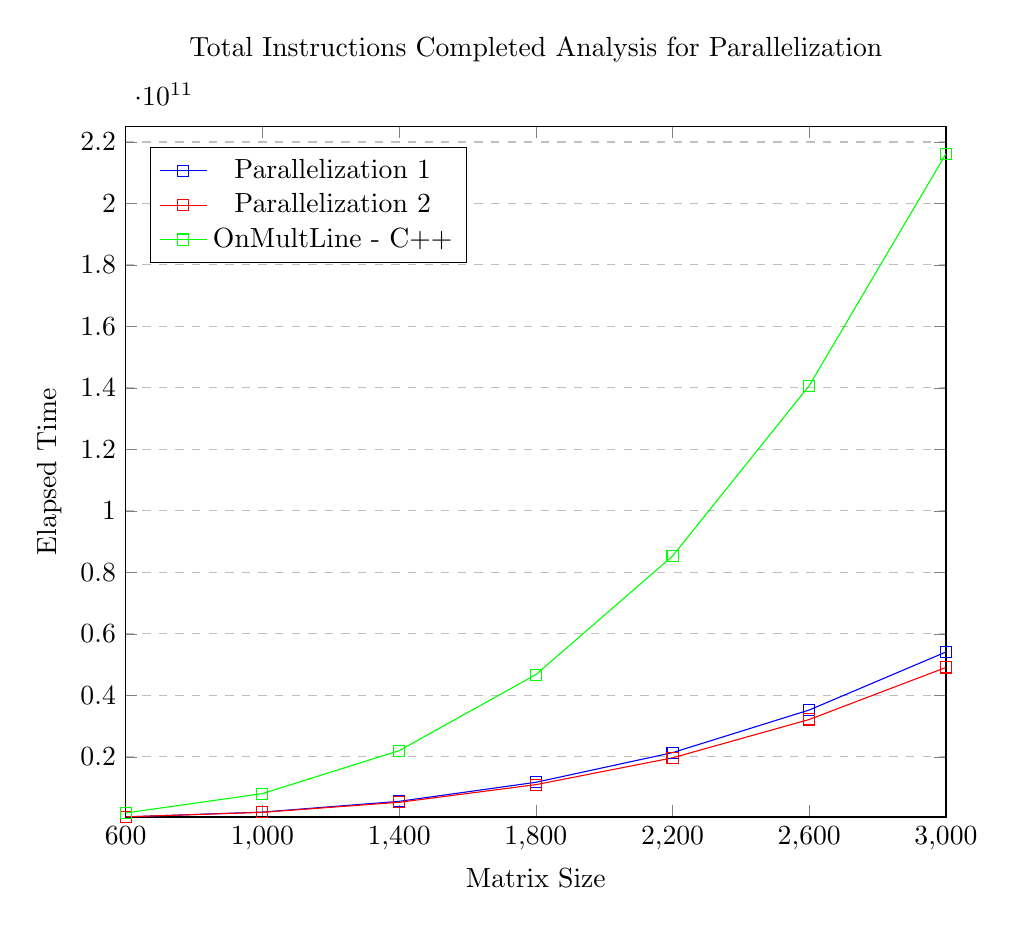
\begin{tikzpicture}
    \begin{axis}[
        title={Total Instructions Completed Analysis for Parallelization},
        xlabel={Matrix Size},
        ylabel={Elapsed Time},
        xmin=600, xmax=3000,
        ymin=400000000, ymax=225000000000,
        xtick={600,1000,1400,1800,2200,2600,3000},
        legend pos=north west,
        ymajorgrids=true,
        grid style=dashed,
    ]
        \addplot[
            color=blue,
            mark=square,
            ]
            coordinates {
                (600,438657212)
                (1000,2013200885)
                (1400,5511784587)
                (1800,11701892016)
                (2200,21351520383)
                (2600,35226846358)
                (3000,54099246852)
            };
        \addlegendentry{Parallelization 1}
        \addplot[
            color=red,
            mark=square,
            ]
            coordinates {
                (600,455248850)
                (1000,1943032002)
                (1400,5195610607)
                (1800,10935697178)
                (2200,19660183111)
                (2600,32140870548)
                (3000,49070275131)
            };         
        \addlegendentry{Parallelization 2}
                \addplot[
            color=green,
            mark=square,
            ]
            coordinates {
                (600,1735286324)
                (1000,8020111511)
                (1400,21991339535)
                (1800,46720971486)
                (2200,85281004166)
                (2600,140743440779)
                (3000,216180278092)
            };
        \addlegendentry{OnMultLine - C++}
    \end{axis}
\end{tikzpicture}
\noindent\rule{\textwidth}{1pt}

% ====================================================================
% Total Cycles Analysis for Parallelization

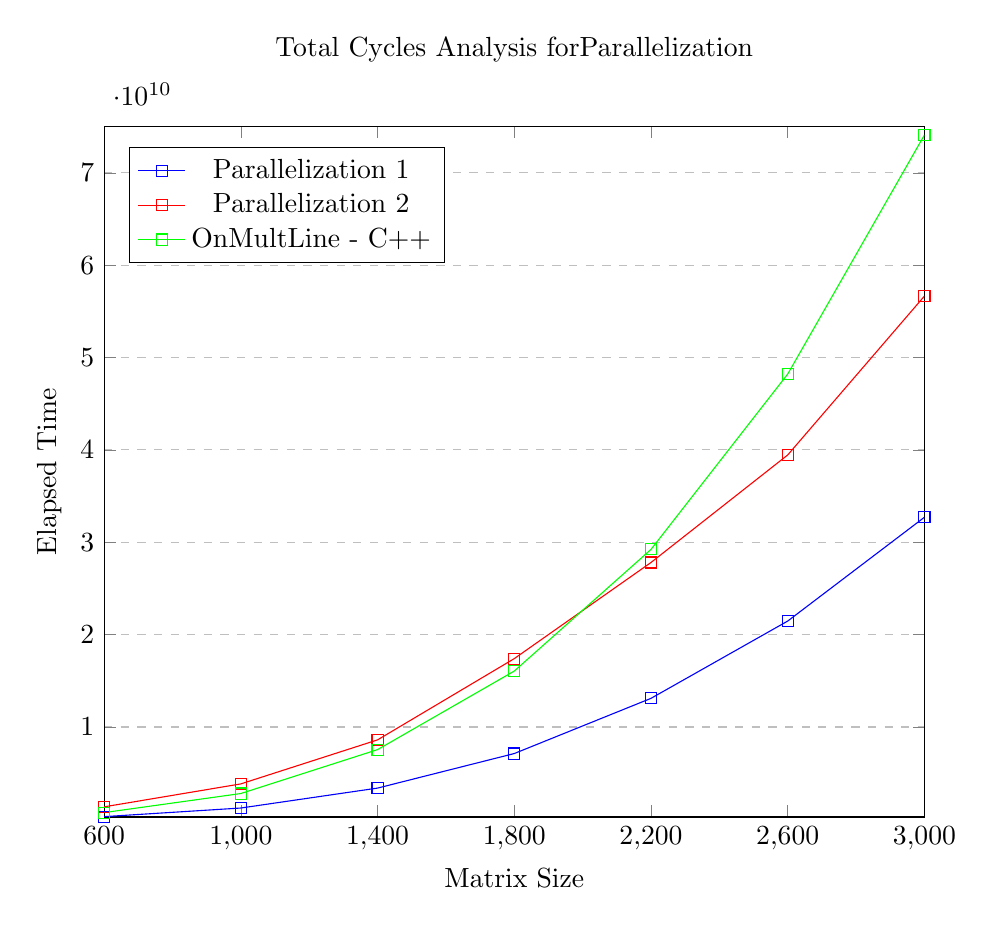
\begin{tikzpicture}
    \begin{axis}[
        title={Total Cycles Analysis forParallelization},
        xlabel={Matrix Size},
        ylabel={Elapsed Time},
        xmin=600, xmax=3000,
        ymin=250000000, ymax=75000000000,
        xtick={600,1000,1400,1800,2200,2600,3000},
        legend pos=north west,
        ymajorgrids=true,
        grid style=dashed,
    ]
        \addplot[
            color=blue,
            mark=square,
            ]
            coordinates {
                (600,293492801)
                (1000,1226473974)
                (1400,3384484947)
                (1800,7124773820)
                (2200,13100888341)
                (2600,21470030132)
                (3000,32708976680)
            };
        \addlegendentry{Parallelization 1}
        \addplot[
            color=red,
            mark=square,
            ]
            coordinates {
                (600,1354166371)
                (1000,3839455172)
                (1400,8603440289)
                (1800,17403267346)
                (2200,27809691934)
                (2600,39452798753)
                (3000,56658331421)
            };         
        \addlegendentry{Parallelization 2}
                \addplot[
            color=green,
            mark=square,
            ]
            coordinates {
                (600,731568849)
                (1000,2796360303)
                (1400,7548688815)
                (1800,16054568787)
                (2200,29225515050)
                (2600,48215845000)
                (3000,74100730666)
            }; 
        \addlegendentry{OnMultLine - C++}
    \end{axis}
\end{tikzpicture}
\noindent\rule{\textwidth}{1pt}

\end{center}

% \section{Título}
% \subsection{Subtítulo}
% \paragraph{Parágrafo}

% \begin{description}
%     \item[Title 1] Description 1
%     \item[Title 2] Description 2 
%     \item[Title 3] Description 3
%     \item[Title 4] Description 4
%     \item[Title 5] Description 5
% \end{description}

% \begin{enumerate}
%     \item enum 1
%     \item enum 2
%     \item enum 3
% \end{enumerate}

% \hl{highlight 1}
% \hl[2]{highlight 2}

% \begin{table}[H]
%     \centering
%     \begin{tabular}{|c|c|c|}
%         \hline
%     \hl{PC} & \hl{IP} & \hl{MAC} \\ \hline
%     TUX63 & 172.16.60.1 & 00:21:5a:5a:75:bb  \\
%     TUX64 & 172.16.60.254 & 00:21:5a:61:2d:df \\
%     \end{tabular}
% \end{table}

% \begin{bash-darktheme}
%     Codigo
% \end{bash-darktheme}

% \begin{figure}[H]
%     \centering
%     \includegraphics[width=0.8\textwidth]{images/part2-exp1.png}
%     \caption{Experiência 1 - TUX64 <-> TUX 63}
% \end{figure}



\end{document}



